%methods chapter
% Enough for an expert to reproduce without needing extensive references
% all data should be in thesis so they can be checked (appendix maybe and supplements)
% Methods commonly used throughout maybe leaving chapter specific methods to that chapter
\graphicspath{{chapters/2.Methods/figures/}}

\begin{savequote}[75mm]
    Science is what we understand well enough to explain to a computer. Art is everything else we do.
    \qauthor{- Donald Knuth: \textit{foreword to \(A=B\) by Petvosek, Wilf and Zeilberger}}
\end{savequote}

\chapter{Methods}

\section{Microbiology}
\subsection{Strain information}
During this project 3 \textit{Paramecium bursaria} cultures have been used.  These have been obtained from 
the UK Culture Collection of Algae and Protozoa (CCAP) and the Japanese National BioResource Project (NBRP).
Specifically:
\begin{itemize}
    \item CCAP 1660/12: \textit{Paramecium bursaria} SW1 with \textit{Micractinium reisseri} SW1-ZK \citep{Hoshina2010}
    \item CCAP 1660/13: \textit{Paramecium bursaria} (unknown strain) with \textit{Coccomyxa} CCAP 216/24 \footnote{This is a mixed culture 
            containing both CCAP 1660/12 strain with \textit{Micractinium} and the \textit{Coccomyxa} bearing strain, 
        the \textit{Coccomyxa} endosymbiont has been further isolated in CCAP under the description CCAP 216/24 (pers. comm. Undine Achilles-Day CCAP)}
    \item NBRP Yad1g1N: \textit{Paramecium bursaria} Yad1w with \textit{Chlorella variabilis} 1N\footnote{
        Yad1g1N host is mating type 1 and was created by mixing of isolated and 
        cultured endosymbiont (\textit{Chlorella variabilis} Clone 1 (known as 1N strain))
        }
\end{itemize}

Both CCAP cultures (1660/12 and 1660/13) were isolated from the same pond in Cambridge, UK (pers. comm. Undine Achilles-Day CCAP, Oban, Scotland)
CCAP 1660/12 was the principal culture and all genomic, transcriptomic and metabolomic analyses were conducted using these cultures. 
Theoretically, these 3 cultures provide us with \textit{Paramecium bursaria} strains harbouring members of 3 of the 4 species of 
green algal \textit{Paramecium} endosymbiont (see Chapter 1 \ref{chap1} for more details).

\subsection{Media and Culture conditions}
All \textit{P. bursaria} and green algae cultures were maintained in 
New Cereal Leaf-Prescott Liquid (NCL) media 
(\(4.3g/l CaCl_{2}.2H_{2}O\), \(1.6g/l KCl\), \(5.1g/l K_{2}HPO_{4}\), \(2.8g/l MgSO_{4}.7H_{2}O\), 
\(1g/l\) wheat bran, gravity filtered via \(GF/C\) paper and autoclaved) \citep{NCLCCAP} and stored in 
an incubator at 15\celsius with a 12:12 light:dark cycle.  The incubator was
lit using 2 \(21w\) 865 daylight fluorescent tubes, producing 2000 lumen each.
Cultures were sub-cultured approximately every 2 weeks using fresh NCL media and were inspected using light microscopy to monitor health.  
No bacteria was added to cultures used for ``omic'' analyses but otherwise the medium was bacterised with
\textit{Klebsiella pneumoniae} SMC (strain donated by the Meyer Lab, Ecole Normale Supérieure, Paris, France) the day before use. 

\section{Omics}
``-omic'' technologies are those aimed at globally characterising a class of biomolecules 
within a specific biological sample (characterising the ``-ome''). The major areas of this
are genomics, transcriptomics, metabolomics and proteomics. 
Genomics aims to characterise DNA and generally involves sequencing the genome, it is used
to discover and describe genes (and non-coding DNA) and by comparison with other genomic
datasets their evolution.  Similarly, transcriptomics is orientated 
around the characterisation of the RNA present in a sample.  This can include
the canonical messenger RNA (mRNA) transcripts but also other RNA elements i.e.
non-coding RNA (ncRNA) such as small interfering RNAs (siRNA) and micro RNAs (miRNA) and
generally involves sequencing the RNA fraction of interest.
Transcriptomics can be used to catalogue transcripts (and their variant splices), 
aid genome annotation,  and/or assess transcriptional response to a given condition or cellular state \citep{Wang2009}.
Metabolomics seeks, instead, to identify and quantify small biomolecules that make up the terminal and
intermediate products of cellular metabolism e.g. carbohydrates, alcohols, and amino acids.  
Finally, proteomics characterises the proteins present in a sample. 
Typically, the metabolome and proteome are interrogated using various forms of mass-spectrometry.
There are also a plethora of additional approaches which seek to characterise
different subsets of these biomolecules e.g. epigenomics (epigenetic modification to DNA such as methylation
and histone binding), gylcomics (characterisation of cellular saccharides).
``Meta-\ldots-omics'' is the application of specific ``omic'' method to a biological sample 
containing multiple organisms. For example, ``metagenomics'' has been used to investigate
the cellular community composition of marine micro-eukaryotes \citep{Cuvelier2010}
and ``metatranscriptomics'' has been used to analyse the transcriptomes of the microbes present in the gut of metazoa \citep{Perez-Cobas2013}.

The utility of ``-omic'' approaches is they allow a researcher to characterise a high proportion 
of a biological system's function in a way that is faster, cheaper and requires less \textit{a priori} 
knowledge of the system than more targeted approaches.
For example, in order to estimate the abundance of all mRNA transcripts in a sample using specific
approach such as RT-PCR would require sequence knowledge to design primers as well as an infeasible amount of
reactions to acquire a characterisation comparable to that obtainable by a transcriptomic approach such as RNA-Seq. 
Additionally, due to being ``non-targeted'' (or rather less targeted) ``omics'' also removes one aspect of 
researched-induced bias caused by a conscious selection of molecule specific probes.
By not considering elements of a system in isolation like the classic methodologically reductionist\footnote{
    Epistemological reductionism: ``explain all biology in terms of physics and chemistry'' \citep{Crick1966}
    i.e. biology is applied chemistry which is applied physics which is applied maths. 
    Ontological reductionism: a biological system is only the sum total of its component molecules and their
    interactions.
    Methodological reductionism: examination of simple components can be used to understand complex system \citep{Fang2011}}
approaches ``omics'' can reveal complex systemic mechanisms/features (or at the extreme ``emergent properties'') that would
otherwise have been missed \citep{Fang2011}.  


However, until relatively recently ``omic'' methodologies were restricted to specialised 
institutions and well characterised ``model'' organisms.  
While, \textit{Paramecium bursaria} and green algae such as \textit{Micractinium
reisseri} could be considered ``model'' organisms throughout the early days of 
molecular biology, they are much less frequently studied in the genomics
era (2000-today) particularly compared to organisms such as \textit{Arabidopsis thaliana} and \textit{Saccharomyces
cerevisiae}. Fortunately, due to the development and maturation of both technologies and databases 
the potential for functional and adaptive analysis of non-model organisms using 
combined ``omics'' (i.e. using genomics as a reference to guide subsequent transcriptomics) approaches 
(e.g. \citep{Munoz-Merida2013,Feldmesser2014}) has recently been demonstrated.  
Additionally, there are two other developments which make \textit{P. bursaria}-\textit{M. reisseri} (\textit{PbMr}) 
increasingly amenable to
``omic'' analysis: \textit{de novo} transcriptomics which dispense with the need to generate
moderately accurate genome in the relatively genomically intractable \textit{Paramecium} (e.g. \citep{Kodama2014}  and
single-cell approaches which allow fine-grained analysis of the \textit{Paramecium bursaria}
- green algal relationship on a cell-by-cell basis.


It should be noted that care must be taken with ``omics'' approaches as they can easily become purely descriptive,
and at worse generate models that lack any biological relevance \citep{Fang2011}.  
This concern holds for all systems-level approaches and has been frequently raised and discussed in the context
of genomics \citep{Dougherty2008}.  Therefore, it is crucial to supplement ``omic'' approaches with targeted
methods in a way that compensates for the weakness of each type of method.
Specifically, the systems approach should be used to generate novel and interesting
hypotheses which can then be tested in isolation using reductionist methods \citep{Casadevall2008}.  
For example, ``omics'' methods could be used to create a model of inter-organism host-endosymbiont
metabolism and targeted approaches such as RNAi could then be used to test hypotheses generated
by this model i.e. testing that a particular transporter protein is responsible
for the transfer of metabolites by knocking out that transporter and observing the resultant phenotype: 
is the relationship perturbed in a predictable manner.

\subsection{Genomics and Transcriptomics}

%\subsubsection{Extracting Nucleic Acids}
%
%The first stage of any genomic or transcriptomic analysis is the extraction
%of nucleic acids from the sample of interest.
%Typically, this involves obtaining large amounts of source biomass either by
%taking large environmental samples and fractionating this using methods like filtration, 
%or flow cytometry or more typically (and with all the biases it involves) establishing
%a culture of the organisms of interest (if possible) and growing that up to sufficient biomass.
%
%For bulk analyses we used a trizol based extraction
%
%For single cell gDNA CTAB \citep{}
%
%material either from a large
%environmental sample or by culturing 
%
%SPADES PAPER HAS GOOD CITES
%While the quality of the output of earlier sequencing techniques
%was highly reliant on both the quantity and quality of the input DNA (or cDNA) (not to mention
%characteristics such as GC\%) precluding many systems from easy analysis.  This is especially
%problematic for the majority of systems that are not easily culturable and thus can't be
%grown up in sufficient quantities to easily extract sufficient nucleic acids to conduct.
%
%Starting with single-cell single-gene sequencing experiments (e.g. \citep{Kuppers1993}) 
%single cell methods allows obtaining data directly from individual cells
%avoiding the bias and complication of culturing or having to decompose a complex environmental
%metagenome or metatranscriptome containing a plethora of diverse cells \citep{Blainey2013}.  It also allows 
%investigation of cells at particular life stages e.g. sexual reproduction without difficult
%and potentially biasing synchronisation methodologies and the sequencing of long genes hard to obtain
%from metagenomes.  
%
%Single-cell genomic (SCG) sequencing has been demonstrated across the tree-of-life as sufficient to infer 
%cellular metabolism \citep{Chitsaz2011}, the dynamics of interactions between organisms \citep{Yoon2011} and
%environmental diversity \citep{Swan2013,Rinke2013}.
%
%Likewise, single-cell transcriptomic (SCT) sequencing has been demonstrated to be an effective tool to investigate
%
%Bulk transcriptomic methods involve analysis of an ensemble of transcripts therefore expression 
%inferences are an average across all cells \citep{Stegle2015}
%
%Sufficient for some purposes, e.g. broad-stroke comparisons it masks the underlying and potentially
%biologically informative stochastic nature of gene expression \citep{Raj2008}.  SCT 
%revolutionises being able to compare different tissues, populations, and cell states in both
%single cell and multicellular systems by allowing direct interrogation of inter- and intra-
%grouping variation and could potentially revolutionise areas such as medicine \citep{Sandberg2014}
%and ecology (Moore Marine Microbe Project \url{http://marinemicroeukaryotes.org/}).
%
%While single cell level analyses have been possible for a while they have largely been restricted
%to low-throughput methods e.g. reporter constructs, FISH etc.
%
%Cell isolation, FACS, microfluidics, cell picking
%
%SCT has relatively high levels of technical noise specifically sampling noise for low-level
%expression and sample-specific variability in sequencing efficiency for highly-expressed 
%transcripts for one SCT method \citep{Grun2014}.
%
%
%mRNA was selected using a poly-A selection method before being fragmented, cleaned-up using ethanol and then 
%reverse transcribed into single-stranded cDNA using random hexamer primers.
%
%Currently, single cell genomics still requires whole genome amplification (WGA) even with 
%3rd generation sequencing platforms due to the relatively inefficient library preparation
%from a single cell (on the range of nanograms). \citep{Blainey2013} %%find support quote for transcriptomics needing WGA too
% 
%Multiple-displacement amplification \citep{Dean2001} is the main method for
%single-cell sequencing.
%REASONS IT IS GREAT
%However, it also generates many biases orders of magnitude differences in coverage
%in different regions 
%SINGLE CELL TRANSCRIPTOMICS ARE SUSPECT
%potential chimeric reads and incongruent read-pairs \citep{Bankevich2012}.
%
%This complicates assembly RODRIQUE PAPER MENTIONED IN SPADES 
%
%E+VSCV paper chisatz 
%
%However, such a different type of data that a new algorithm was needed not just modificaitons \citep{Bankevich2012}
%
%Paired-end data typically only used post-processing step of de-Bruijn graphs.
%Proper use of pairing information at the graph assembly phase is a potential 
%source of improvement.
%2011a medvedev PDBG but fixed insert size
%
%Idury and waterman DBG for assembly: originally considered infeasible as low coverage
%sanger even qitrh few errors needs error correction
%
%Pezner A-bruijn graphs
%everything else special case
%
%
%Single cell methods use multiple-displacement amplification to increase the concentraion of
%nucleic acids 
%
%For example. the Qiagen Repli-G kit used for both single cell transcriptomic and genomic analysis
%of the \textit{PbMr} system.
%
%Transcripts are reverse transcribed and then ligated into larger fragments.  MDA
%is then undergone on the larger fragments before the usual library preparation process.
%
%One interesting consideration for single cell transcriptomics is the possible generation
%of chimeric reads that will cross the boundary between two randomly ligated transcripts.
%
%However, the risk of this can largely be mitigated by selection of a relatively small fragment
%size for paired end sequencing.
%
%5'-3' - 5'-3'  - sequencing primers are unlikely to rpim

\subsubsection{DNA sequencing}

In the majority of cases, genomics and transcriptomics are both synonymous with
the sequencing nucleic acids. Earlier approaches, based upon the fluorescent
marking of the hybridisation of DNA and/or RNA to arrays of short complementary probes 
e.g. genomic tiling arrays and the transcriptome microarrays \citep{Mockler2005}, are of more
limited utility.   Relative to sequencing-based approaches these methods
require relatively more prior knowledge of the organism and require a custom array to be
designed for any novel system. Additionally, while microarrays can determine relative expression levels
of transcripts by the comparison of the fluorescence intensity at given complementary probe(s)
the continuous nature of this output, difficulty distinguishing alternative isoforms 
and more limited dynamic range (combined with previously mentioned limitations) 
has meant the sequencing of cellular transcripts (RNA-Seq) has largely supplanted microarrays \citep{Wang2009}.
However, both SNP tiling arrays and microarrays do have the advantage of throughput and ease of analysis
in situations where the host organism is well known and suitable arrays have already been designed
and evaluated.  For this reason they are still frequently encountered in specialist area of medical 
diagnostics.


While it is possible to directly sequence RNA transcripts \citep{Ozsolak2009} most approaches first utilise a reverse transcription (RT)
step to convert transcripts to cDNA. As ribosomal RNA makes up a sizable proportion of RNA in the cell
it is often necessary to enrich or select the RNA fraction of choice in order to minimise wasted effort when
sequencing \citep{Wilhelm2009}.  For eukaryotic mRNA enrichment this can be easily achieved by
using poly-T primers during RT which selectively bind to the poly-adenylated tail of these messenger 
transcripts.  However, for bacterial/archael work and transcriptomic analyses focussing on non-poly-adenylated
transcripts such as ncRNAs/siRNAs/miRNAs etc. ribosomal depletion is used \citep{ONeil2013}.  This is a process by which 
ribosomal probes are attached to magnetic beads. Ribosomal RNAs bind to these probes and the magnetic
beads can be used to partition the majority of ribosomal sequences away from the other RNA \citep{ONeil2013}.
This means that transcripts can be sequenced using the same methods and platforms as any other DNA sample with analysis only diverging against post-sequencing.
It should be noted that there are potential disadvantages to this reverse transcription step and it
can potentially generate artefacts and biases in the analysis (as well as placing limitations on the quality
and quantity of input RNA) \citep{Ozsolak2011} however, the advantages of the more developed DNA sequencing technology outweighs these
disadvantages.

% "as such replication is important" tom note??


These DNA sequencing technologies can largely be divided into 3 technological eras with today (2015) 
broadly at the transition between 2nd and 3rd generations.


1st generation (also known as Sanger) sequencing technology originated in 1970s with the work of Sanger \&
Coulson \citep{Sanger1975,Sanger1977,Sanger1977a} which 
developed sequence determination via the principal of chain termination during 
synthesis and subsequent determination of relative fragment sizes. 
Briefly, by having 4 separate reactions in which DNA synthesis terminates on the incorporation
of dideoxy nucleotides (ddNTP) corresponding to each of the 4 principal DNA bases (i.e. ddATP, ddGTP etc.) 
you can generate a series of DNA fragments of various sizes.  Size fraction separation of these fragments 
via methods such as gel electrophoresis means the DNA sequence can be easily read from the fragment size distribution
across the 4 ddNTP reactions \citep{Sanger1977a}. 
This technique was used to sequence the first DNA genome (bacteriophage \(\phi X174\) \citep{Sanger1977}).
The methodology was subsequently improved by use of fluorescently labelled ddNTPs by Leroy Hood,
massively simplifying automation of the process \citep{Smith1985,Smith1986}.
Further improvements followed throughout the 1990s and early 2000s such as capillary electrophoresis
and other general throughput and length enhancements \citep{Bonetta2006}.
Transcriptomic analysis was possible using Sanger sequencing by generating clone libraries from partial or complete cDNA and randomly sequencing
clones \citep{Adams1991,Gerhard2004}.  However, while this did allow resolution of different isoforms and could be used to aid annotation \citep{Adams1991}
it was not possible to investigate relative expression levels beyond a broad identification of highly expressed transcripts based on the 
proportion of the cDNA/EST library they made up.
Sanger sequencing's main utility lies in high quality short fragment (\(300-1000bp\)) sequencing to determine or confirm the sequence 
of specific DNA fragments such as vectors or PCR products \citep{Bonetta2006,Tsiatis2010}.  


2nd generation sequencing emerged commercially in 2005 with the work
of both George Church and 454 Life Sciences \citep{Margulies2005} and featured
reduced individual reaction volumes, greater parallelisation (and so higher throughput),
cell-free preparation without the need for time-consuming cloning of DNA fragments into bacterial vectors to generate
clonal templates for sequencing, and direct sequencing detection obviating the need
for size fractionation \citep{Jaszczyszyn2014}.
These technologies generate huge amounts (on the order of \(10^{6}-10^{9}\) of relatively short (on the order of \(10^{1}-10^{3}bp\)) DNA sequences 
    (reads) randomly sampled from the input (c)DNA. 


Commercially available 2nd generation platforms include 454's GSLFLX and GSJunior (now Roche),
Ion Torrent's (now Life Technologies) PGM, Applied Biosystem's (now Life Technologies) SOLiD and Illumina's (formerly Solexa) 
HiSeq, MiSeq and older Gene Analyzer II \citep{Nederbragt2012}.

\begin{figure}
    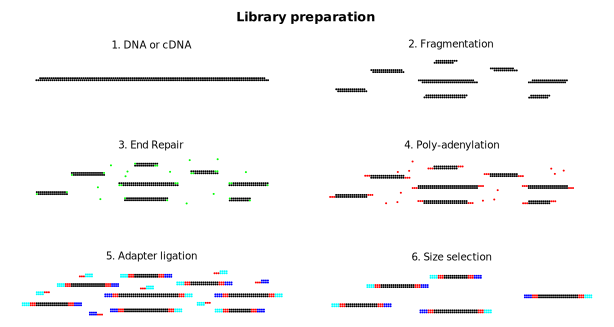
\includegraphics[width=\textwidth]{illumina_lib_prep.pdf}
    \label{fig:libprep}
    \caption[Illumina Library Preparation]{A brief overview of library preparation for Illumina modified from \citep{Mardis2008} and Illumina TruSeq kit documentation} 
\end{figure}

Although these platforms use a range of different implementations and tend to exhibit various different trade-offs (mainly in terms
of number of reads and their respective lengths) they all largely follow the same basic process \citep{Shendure2008}:
\begin{enumerate}
        \item Library generation: Randomly fragmenting input DNA into short fragments of a specific size
            followed by ligation of adapter sequences with some platforms allowing development of ``paired-end'' or ``mate-pair'' libraries in which
            each end of a fragment is sequenced separated with a known size unsequenced fragment aiding subsequent assembly (see \ref{fig:libprep})
        \item Clonal amplification: Generation of clonally identical spatially distinct clusters of DNA mainly via emulsion PCR \citep{Dressman2003} (SOLiD, Ion Torrent, 454)
            or bridge PCR \citep{Adessi2000,Fedurco2006} (Illumina) (see \ref{fig:libseq})
        \item Sequencing-by-synthesis: In which a complementary DNA strand is generated base by base via sequentially flooding and clearing a
            chamber with each dNTP and a polymerase (or ligase in the case of SOLiD).  On incorporation of a base into a cluster a detectable signal is released such as emission of certain wavelengths of light 
detectable using optics (e.g. Illumina, 454, SOLiD) or release of hydrogen ion (e.g. Ion Torrent).
\end{enumerate}

The explosion in sequencing throughput on 2nd-generation platforms has driven a massive decrease in per-base sequencing cost
and the subsequent expansions in the amount of available data (e.g. the US National Center for Biotechnology (NCBI)'s short-read archive (SRA)) 
has made both genomic and RNA-Seq analysis and annotation easier and more effective. 

\begin{figure}
    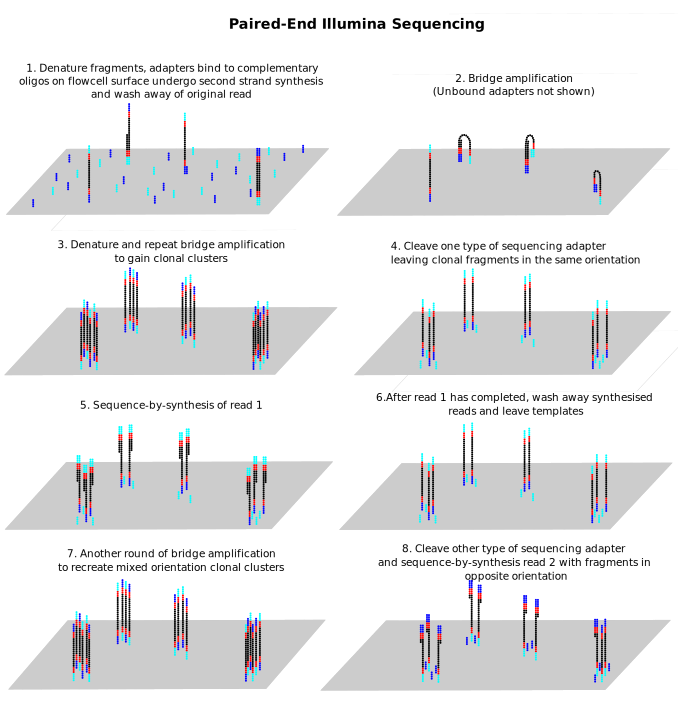
\includegraphics[width=\textwidth]{illumina_PE_sequencing.pdf}
    \label{fig:libseq}
    \caption[Paired-end Sequencing]{A brief overview of paired end sequencing in an Illumina flowcell after library preparation, derived
    from \citep{Mardis2008} and Illumina}
\end{figure}

While, 2nd generation sequencing has driven down per-base sequencing costs the cost of library preparation 
has fallen more slowly \citep{Blainey2013}.
For this reason, combined with the higher throughput it has become common to multiplex difference samples 
during sequencing runs.  Multiple distinct samples can be be sequenced
in the same reaction (e.g. flowcell lane for Illumina platforms) by adding an indexed tags during library
preparation.  These tags can then be used to partition the reads back to their original separate samples
after sequencing. 

The current \textit{de facto} standard in 2nd generation sequencing is that of the bridge amplification
based \citep{Shendure2008} Illumina platforms \citep{Regalado2014} due to relatively low error rate (\(\leq0.1\%\) \citep{Glenn2011}),
very high throughput (e.g. HiSeq2500 generates up to 400M 125bp reads per run (1TBase of data) \citep{Nederbragt2013})
and the lowest cost per Mb (\(\leq\$0.04\) \citep{Glenn2011}).


Finally, 3rd generation technologies are generally known as single-molecule sequencing.
These platforms sequence individual DNA (or RNA molecules \citep{Ozsolak2009}) without
bias and error-prone amplification. 
The first 3rd generation platform was that of the now defunct Helicos Bioscience's Helicoscope \citep{Harris2008}
based on breakthroughs in the resolution of fluoresence visualiation using paired FRET methods \citep{Braslavsky2003}.
There is only one publically available platform: Pacific Biosciences (PacBio) RS platform. PacBio operates on a similar principal
of sequencing-by-synthesis as the 2nd generation platforms but uses fixed polymerases at the base
of specially wave-guide structures allowing the detection of fluorescence from a single reaction
instead of many parallel reactions in a clonal cluster.  This produces few (compared to 2nd generation 
platforms) long (20kb and longer) reads but has a high cost and high error rate (14\%) \citep{Jaszczyszyn2014}
Another platform, currently in testing, Oxford Nanopore's MinIon, reads individual strands of DNA through an array of 
pore proteins and determines the sequence at each pore based on the physical
properties (impedance) of a particular set of bases.

Unfortunately, partly as an element of their relatively nascent state and partly due to the
poorer signal:noise of single molecule approaches compared to analysing large 
batches of identical DNA sequences, 3rd generation technologies have a relatively high error rate.
Thus are generally inadequate for most eukaryotic assembly tasks in and of themselves.
Where they have shown great utility is in conjunction with 2nd generation datasets
as a scaffolding tool i.e. producing long noisy reads upon which more accurate but shorter
reads can be assembled.


Therefore, all genomic and transcriptomic sequencing in this PhD has been performed using the 2nd generation
Illumina HiSeq platform due to its relative maturity, high-throughput, relatively accurate
paired-end output making it currently the most amenable platform to effectively
use \textit{de novo} genomic and transcriptomics approaches.  Additionally, Sanger sequencing
has been used when accurate targeted sequencing was called for, such as investigating the
taxonomic distribution of \textit{Paramecium} green algal endosymbionts (see \ref{chap1}).


\subsubsection{Read pre-processing}

Read pre-processing is a key stage in the assembly of next generation sequencing data regardless of the assembly
methodology used. 

Typically, this involves 4 key steps:
\begin{itemize}
    \item Library quality control and contamination screening
    \item Trimming sequencing adapters and low probability reads
    \item Error corrections
    \item Digital normalisation
\end{itemize}


Arguably, trimming, error correction and normalisation are all aspects of the same process.


The specific error correction algorithms are largely based on the assumption that sequencing errors
are infrequent and randomly distributed 




Trimming

Error correction algorithms 

normalistion




\subsubsection{Assembly}

There are two main approaches to both genome and transcriptomic assembly - referenced and \textit{de novo}.
A referenced assembly consists of the alignment of processed reads 

\subsubsection{Differential expression}

Comparison of different methods of normalisation \citep{Dillies2013}




%\subsubsection{Assembly}
%
%All major 2nd and 3rd generation sequencing platforms output a FastQ formatted file.
%These are files containing the sequence of a read and a per-base quality score known as a Q score.
%These scores (Q) are calculated as a logarithmic relation to the base-called error probability (P)
%\[ Q = -10\log{10}{P} \]
%and conversely: 
%\[ P = 10^{frac{-Q}{10}} \]
%Therefore \[Q = 30 \] corresponds to 99.9\% base call accuracy
%
% mapping reads to reference can introduce biases even with relatively \citep{Wang2012}
% but even if the reference is divergent it may still produce a higher quality assembly
% than de novo methods \citep{Vijay2013}
% Soap-denovo trans and trinity performed better than transabyss \citep{Vijay2013}
% In De Bruijn graph assembly generated from exact subsequence matches - errors exponentially increase
%possible graph traversal paths increasing graph comp-lexity and assembly time and memory \citep{Pop2009}
%
%
%https://www.biostars.org/p/52178/ sequencing papers theory
%Spades \citep{Bankevich2012}
%
%Trinity \citep{Grabherr2011}
%
%\subsubsection{Trimming}
% Hard filters can improve assembly and mapping but will likeluy lose lowly-expressed transcripts \citep{MacManes2014}
%\subsubsection{Error correction}
% Error correction of Illumina sequencing reads has been acknowledged as an increasingly important step in the
% creation of both genomic \citep{Schatz2012a} and transcriptomic \citep{Macmanes2013} high quality assemblies.  
% Difficult for transcriptomic datasets (and SC) because can't rely of varied coverage \citep{Macmanes2015}
% Under 50M reads bfc is best, more than 50M seecer is better and if research is sensitive to erroneous correction Lighter is best \citep{Macmanes2015}
% Seecer developed explicitly for RNA-Seq

%There are many available tools for read-trimming (as discussed in the Methods Chapter),
%and a range of trimming tools were initially
%considered: specifically Trimmomatic \citep{Bolger2014a}, Sickle \citep{JoshiGitHub}, FASTX-toolkit \citep{gordon2010fastx},
%PRINSEQ \citep{Schmieder2011} and cutadapt \citep{martin2011cutadapt}. 
%Despite Sickle, an adaptive quality trimmer, having previously been used in single-cell transcriptome datasets 
%from free-living eukaryotes \citep{Kolisko2014}, it proved suboptimal as it was
%not capable of removing 5' or 3' contaminants such as sequencing adapters and/or multiplexing tags by itself.  
%These stages could be achieved with individual tools (such as Skewer \citep{Jiang2014}, 
%TagDust \citep{Lassmann2009} and Scythe \citep{Buffalo}) but this was rejected as it was
%deemed a needless complication.  Furthermore, Sickle proved to be relatively poorly documented
%as a tool.   As for other trimming tools, they mostly have  
%been found to largely perform equivalently across multiple RNA-Seq and DNA-Seq datasets and applications 
%(see File S2 \citep{DelFabbro2013}).  Additionally, cutadapt requires either manual repair of 
%paired read correspondence or discards all reads that are unpaired after trimming. It also requires
%use of ancillary shell scripting to input all desired adapter sequences from a sequencing service
%provided adapter fasta file.  Similarly, neither PRINSEQ or FASTX are competent to trim paired-end datasets 
%natively requiring work-arounds to retain pairing fidelity.
%Therefore, due to its advantages of maintaing read-pair correspondence during trimming, 
%optimisation for Illumina datasets, adapter trimming functionality and thorough documentation
%Trimmomatic \citep{Bolger2014a} proved the preferred trimming tool for this analysis.

% Cluster kmers - then mininmise size of kmers clusters: kmer-spectra, suffic array, MSA, and HMM
% Methods reviewed here \citep{Molnar2014}
% A key component of the Spades single cell genomic assembler is the error correction using Bayeshammer 
% SCT have very non-uniform coverage \citep{Nikolenko2013}
%

%
%\subsection{Assessing Assemblies}
%
%RSEM-eval, mappings, NG50, L50, N50
%    
%
%Assemblathon 1 \citep{Earl2011}
%GAGE \citep{Schatz2012}
%Assemblathon 2 \citep{Bradnam2013}
%Nucleotid.es: Linux Container (specifically Docker \citep{Merkel2014})  based continuous assembly evaluation using QUAST \citep{Gurevich2013a})
%

%\subsubsection{The Problem with Ploidy}
%
%One important complication in the assembly on eukaryotic genomes 
%relative to bacteria or archael sources is the issue of highly heterozygous polyploid genomes.
%This is problematic as the de Bruijn graphs constructed during assembly
%rapidly increase in complexity when reads from heterozygous samples become
%incorporated \citep{Kajitani2014}.  This is because k-mers derived from heterozygous regions of 
%homologous chromosomes will partition the assembly graph into bubbles that cannot be easily 
%or accurately resolved by most assemblers expecting only limited structural variation during
%assembly.  Previously, attempts to work around this included inbreeding to generate
%homozygous lines or fosmid based approaches.
%
%Specialised genome assemblers have been produced to address this problem,
%for example Platanus performed well on both highly and lowly heterozygous 
%genomes using k-mer autoextension approaches and by merging haplotypes
%at both contig assembly and scaffolding steps, as well as incorporation
%of various heuristics involving bubble resolution \citep{Bradnam2013,Katjitani2014}
%
%Likewise, transcriptome assembly complexity rapidly increases with the number of alleles
%expected per gene determined by ploidy, heterozygosity and complex gene families
%and in turn how many transcripts per allele in light of alternative splicing.
%
%This is particularly problematic in the PbMr system owing to the massive
%ploidy of the host \textit{Paramecium bursaria} and the numerous whole genome
%duplications in its relatively recent evolutionary history (1).  This also 
%explains the difficulties in using sister species, as the most sequenced Paramecium
%genus species are the aurelia complex which have undergone 2 WGD since divergence with
%\textit{P. bursaria} \citep{McGrath2014}.

%\subsubsection{Genomics}
%Project standards:
%Standard Draft: Minimally filtered, incomplete, assembled into contigs, may have poor regions and be incomplete, may have some contamination
%High-quality Draft: coverage of at least 90\% of genomes or target regions, contamination exluded, little manual review, still might be seq errors or misassemblies, no implied order and oreintation to contigs (can be assessed for gene content)
%Improved-high quality draft: manual or automated additional work, gap resolution, no obvious missassemblies, normally adequate for comparison with other genomes
%Annotated-Directed Imrpovement: Overlapping, improved with annotation, verified, gene models etc useful for gene comarpsiosns, alt splicing, pathway reconstruction
%Noncontiguous finished: high quality, finished apart from a few repeats or gaps, good enough for almost all analayses
%Finished: gold standard, less than 1 error per 100,000, replicon in contig seqs, reference quality \citep{Chain2009}


%\subsubsection{Annotation}
%
%Reed \textit{et al.} \citep{Reed2006} divided components annotation into a useful dimension paradigm as follows:
%\begin{enumerate}
%    \item Enumeration: identification of genes and assignment of their predicted or known functions. What?
%    \item Interaction: integration of protein-protein, regulatory and metabolic interaction data between components Can they interact?
%    \item Genomic Localisation: analysis of genomic localisation of genes i.e. epigenetics.
%    \item Plasticity: investigation of the change of other dimensions over evolutionary time. Does their interaction change over time? \citep{Reed2006} 
%\end{enumerate}
%
%Clearly, at a systems level it is difficult (if not impossible currently), 
%even in well defined model organisms, to complete a full 4-dimensional annotation 
%for all cellular components. However, it is more than feasible to have a largely
%complete 1D and even 2D annotation with 3D and 4D investigated for specific 
%components.  Furthermore, annotation can be conducted with a range of confidences
%from in silico predicted interactions to biochemically validating those predictions in vivo
%and incorporating the precision and recall of various methodologies. Generally, such a process
%is inherently iterative with successive model building and experimental testing and validation 
%or rejection of such models \citep{Reed2006}.
%
%One of the major goals of this thesis is to reconstruct a preliminary predicted
%2D annotation of the PbMr system.
%
%The most important step towards this goal is that of eukaryotic gene prediction.
%
%Eukaryotic gene prediction is achieved by generally two methods - \textit{de novo} HMM based
%methodologies (e.g. GENESCAN, TWINSCAN \citep{}<++>) and expression evidence based methods
%in which reads from sequenced cDNA (or in older approaches ESTs) are aligned to the 
%assembled genomic contigs \citep{Brent2007}.  Unfortunately even relatively deep
%sequencing of cDNA can fail to identify the structure of 20-40\% of genes in a typical
%eukaryote genome owing to these genes being expressed only at very low levels or in
%different conditions than that from which the cDNA was extracted \citep{Brent2007}.
%
%
%
%\subsection{Transcriptomics}
%While generally computationally simpler than genomic assembly \citep{MacManes2014}
%owing to the relatively fragmented nature of transcripts compared to genomic 
%sequences (i.e. lots of transcripts of various lengths rather than several 
%long chromosomes).  There a few key challenges to transcriptomic assembly
%that is absent in genomic work specifically:
%\begin{itemize}
%    \item Handling assembly of alternative isoforms of transcripts \citep{Pyrkosz2013}
%    \item Assembly of transcripts from gene-dense genomes with overlapping 5' UTR 
%    \item Assembly of data with highly heterogeneous read coverage, as transcript
%        expression level is proportional to read coverage (indeed expression analysis
%        using RNA-Seq datasets relies upon this fact).
%    \item Random hexamer bias
%    \item GC content bias, particularly so in PbMr
%\end{itemize}
%
%These problems are particularly problematic in \textit{de novo} approaches,
%however referenced assembly has its own issues in transcriptomics
%
%
%
%
%
%
%
%
%
%
%
%The correlation of transcript level to protein level is difficult
%
%
%
%
%
%Unfortunately, conventional RNA-seq requires either an established moderate-to-high
%density culture of the organism of interest 
%
%
%
%
%
%
%
%
%http://rnaseq.uoregon.edu/
%http://bioinformatics.bc.edu/marthlab/scotty/scotty.php
%
%Experiemntal design, read depth, ENCODE, Tarazona S 2012 fdiff exp in RNA-seq
%a matter of depth
%
%\begin{itemize}
%    \item Check Quality (FASTQC)
%    \item Trim reads (Trimmomatic)
%    \item Re-check quality (FASTQC)
%    \item Error-correct reads (?)
%    \item Normalize coverage (khmer)
%    \item Test paramters for multiple assemblers
%    \item Run each assembler with best parameters
%    \item Analyse all and merge best assemblies
%    \item Annotate transcriptome
%    \item Map reads to assembly, count
%    \item Differential expression analysis
%\end{itemize}
%
%
%
%
%
%
%
%
%
%
%Further complications from single cell:
%Fusions are created in cDNA ligation step prior to MDA in WTA
%However, poly-A tails should mean fusion reads are unlikely as they need to a
%span poly-A trac in all 4 possible fusions apart from 3'-5':5'-3'
%So to get high levels of chimeric reads we would need the two same transcripts
%in the same fused orientation multiple times.  Otherwise any other 3'-5':5'-3'
%fusions should be fairly rare so likely discarded in error-correction etc steps
%
%\subsubsection{Quality Checking}
%
%FastQC tool and its parameters
%
%\subsubsection{Read trimming}
%
%% /storage/fin/raw_reads/raw_sct_reads/optimising_trimming_paramters/test_mapping_to_bulk
%
%
%Currently, there is no clear answer to the question, which is the best trimming algorithm.
%This is due to many dataset-specific effects as well parameter-dependence \citep{DelFabbro2013}.
%However, 
%
%
%
%Trimming algorithms can be divided into two groups: running-sum based approaches e.g. Cutadapt and ERNE-FILTER
%and window-based e.g. FASTX, PRINSEQ, Sickle and Trimmomatic \citep{DelFabbro2013}.
%
%
%
%
%
%
%
%
%
%
%
%
%Difficulties: 
%A major source of bias in transcriptomic datasets is that of compositional biases induced
%by the random hexamer priming used in the generation of cDNA in many library preparations.
%(see \ref{}<++>) %previous section of sequencing itself %does SCT kit do random hexamers?
%Specifically, these random hexamers do not bind uniformly across the transcripts,
%therefore the location of reads are not uniform \citep{Hansen2010}\citep{Hansen2010}.
%Fortunately, the single cell kits do not utilise random hexamer priming {}<++> %Check with DAVID
%So despite inducing other biases, they do not induce this one!
%
%
%Another source of bias is the strong correlation between GC richness in read coverage
%observed in 2nd-generation Illumina sequencing \citep{Dohm2008,}
%This is possibly to do with the different biophysical properties of GC-rich dsDNA (high melting point) \citep{Dohm2008} %is this relevant?
%Or biases in PCR -ampligication, or specifically i9n bridge PCR of cluster amplification
%
%
%Errors are more common at the start and end of 
%
%
%
%
%Sequencing errors: Illumina sequencing has non-random error distribution across length of read, increasing towards the 3' end liu2012. These errors are generally substitution errors yang2013 at a rate of 1-3\% globally \citep{MacManes2014}.  However, while the latest assemblers (see \ref{}<++>) are capable of %ref to assembly section
%handling many of these errors, inevitably sequencing error does cause some
%assembly error MacManesANDEISEN2013.
%Furthermore, errors rapidly increase both the space and time complexity of the assembly (discussed in \ref{}<++>) problem \citep{MacManes2014}.
%
%One of the most important and prevalent methods to try and improve assembly
%accuracy in the face of sequencing errors is that of read trimming, typically
%using one of a range of tools: TRIMMOMATIC, SICKLE, FASTX-TOOLKIT, BIOPIECES \citep{}<++>. %citations for tools
%
%Trimmomatic is the preferred tool of choice as it more read-pair aware than
%FASTX-TOOLKIT and BIOPIECES, retaining pair ordering and conducting more
%advanced trimming checks using pairing information such as adaptor read-through.
%By retaining pairing information and outputting ``surviving'' paired reads and
%unpaired reads TRIMMOMATIC precludes lengthy repairing of header pairing information
%in large datasets. \citep{}<++> %More information about how trimmomatic oworks and comparison to other trimmers
%
%The main approaches used individually or as a combination in trimming tools are that 
%of adaptor trimming (identifying and removing sequencing adapter sequences from reads),
%sliding windows (removing nucleotides that fall below a provided average quality threshold),
%basic terminal quality trimming (remove individual 5' or 3' nucleotides that have an associated PHRED score
%below a ceratin threshold) and minimum length (discard reads that fall below a minimum length). 
%\citep{}<++> %citations explaining these methods
%
%The key difficulty is that all widely used tools above require user-defined thresholds
%for the various trimming parameters e.g. for sliding window approaches - a window size
%and a minimum average quality threshold over the window.  
%This leads to a careful trade-off, if conservative/aggresive (i.e. high) quality thresholds
%are used many reads will be discarded, reducing the amount of data from which to 
%construct an assembly.  This will reduce feature resolution such as alternative splices 
%and in will lead to the loss/reduced assembly accuracy of lowly expressed (but potentially biologically interesting) transcripts \citep{MacManes2014}. On the otherhand, instinctually if permissive (i.e. low)
%quality parameters are set then potentially erroneous reads will be incorporated into the assembly
%and global assembly accuracy will decline. 
%
%Relatively little work on the optimisation of these parameters has been conducted, and generally
%researchers conducting high-profile \textit{de novo} assemblies utilise aggressive thresholds \citep{MacManes2014}.
%However, for \textit{de novo} transcriptome assembly assessed using a range of metrics
%(e.g. mismatches to previous datasets, kmer number, PE reads mapping back to assembly etc.)
%most of the gain of assembly accuracy occurred at a threshold of \(\geq 5\).
%Particularly, low abundance kmers are largely discarded with a threshold of \(\geq 5\).
%Suggesting, that a very low threshold of 2 or 5 optimises assembly quality potentially
%followed by kmer abundance based error correction \citep{MacManes2014}.
%
%
%
%% TRY THIS FOR SCT
%
%
%
%
%
%
%
%
%\subsubsection{Error correction}
%
%While second-generation sequencing technologies have massively increased
%throughput on an individual read basis they exhibit a much higher error
%rate than earlier Sanger approaches with Illumina HiSeq reads showing \(0.5-2.5\%\)
%error rate \citep{Kelley2010}.  
%
%These errors complicate assembly as they will rapidly increase
%the complexity of the de-Bruijn graphs 
%
%Typically the most widely used error-correction algorithms for 2nd-generation
%sequencing reads. 
%
%
%While explained later in \ref{Assembly}, generally OCC assembly is reliant on 
%fast and accuarte overalp calculations while de Bruijn approaches require
%robust error correction \citep{Palmer2010}.
%
%
%
%Single-cell genomics sequencing reads display high variance in their coverage 
%across the genome with some sections. Previously error correction tools (such as
%QUAKE \citep{Kelley2010}
%
%\citep{Nikolenko2013}
%
%Sequence error correction improves \textit{de novo} assembly \citep{MacManes2013}
%
%
%
%
%
%
%
%
%
%\subsubsection{Digital normalisation}
%
%\subsubsection{Assembly}
%Optimising parameters
%Theory
%Combining
%
%
%Almost every \textit{de-Novo} assembly algorithm use one of two approaches:
%overlap-contig-consensus (OCC) e.g. Celera etc
%de Bruijn is more widely used but even as recently as 2010 it was unclear
%which approach was superior \citep{Palmer2010}.
%However, it has become rapidly evident with further expanding sequencing capacity
%
%
%
%
%
%Assembly assessment:
%Adapter trimmed PE reads concordantly mapping to assembly \citep{MacManes2014} 
%Number of complete ORFs (start and stop codons) using TRANSDECODER 
%Unique transcript number using BlastP (80\% similarity over 100aa and e-10)
%%Expression for each contig https://github.com/macmanes/trimming_paper/tree/recreate_ms_analyses/scripts
%
%
%\subsubsection{Annotation}
%
%\subsubsection{Mapping}
%
%The tradeoff between read-mapping sensitivity (number aligned) and specificity (number correctly aligned)
%Modern aligners overcome most errors making trimming unecessary \citep{DelFabbro2013}
%
%
%
%
%
%However, studies on simulated datasets have shown that the main sources of error
%when conducting mapping to a reference transcriptome to infer expression counts
%the most important sources fo error are splice variants and missing transcripts
%\citep{Pyrkosz2013}.  Interestingly, this paper also found that different mapping
%strategies did not yield substantial differences in mapping quality \citep{Pyrkosz2013}.
%
%When mapping RNA-Seq data there is diminishing returns with 1M reads providing 
%approximately the same level of accuracy in estimate transcript abundance 
%as >30M reads for highly-expressed gene in six standard model organisms \citep{Lei2014} 
%
%
%\subsubsection{Transcriptomic Analysis}
%
%The first stage in an analysis of expression is the mapping of
%RNA-Seq reads to the transcripts (whether these have been derived
%from \textit{de novo} assemblies and/or genome annotations).
%This produces a set of digital counts for each transcript, approximately
%in proportion to its relative expression level.
%
%This mapping is done with any of many short-read alignment algorithms
%which are optimised for both speed and accurately mapping short queries (i.e. reads)
%to longer databases (transcriptome/genome) (see \citep{Fonseca2012} for a review of
%tools).
%
%This is true for both bulk and SC RNA-Seq \citep{Stegle2015}.
%
%
% \subsubsection{Transcriptome Assembly Assessment}
% who could http://www.ccforum.com/1471-2164/14/465 \citep{Neil2013c}

% Reference-free assessment is more difficult. 
%   How does RSEM-Eval work \citep{Li2014}
% RSEM-EVAL for an assembly \(A\) and set of reads \(D\)
% \(Score(A) = log P(A, D)\) 
% log P(A,D) = log \int 
%Mapping reads to 


RSEM-EVAL uses the concept of a latent true assembly for a given set of 
reads.  Li et. al. define this as 

For each read r, transcript(r) is the transcript, left(r) and right(r) are the 5' and 3' prime
positoon of the transcript 

a transcript is true if 


\subsection{Metabolomics}

Metabolomics revolves around the detection and characterisation of cellular metabolites via a range of techniques.
By qualitatively and/or quantitivately analysing these molecular substrates, cofactors and products of cellular metabolism
a researcher can determine cellular state or response at the level.

Metabolites are direct signatures of biological activity \citep{}


It is the final level in the path that links genotype to cellular phenotype \citep{Fiehn2002}



Mteabolomics can range from target analysis (focussing on a single metabolite) to 
metabolic profiling (orientated on the metaboites of a specific pathway or type) to
full metabolomics (uuntargeted analysis of the entire metabolome) to metabolic fingerprinting
(high throughput metabolomics of a large number of organisms, also sometimes referred
metabonomics) \citep{Fiehn2002}.




\begin{figure}
    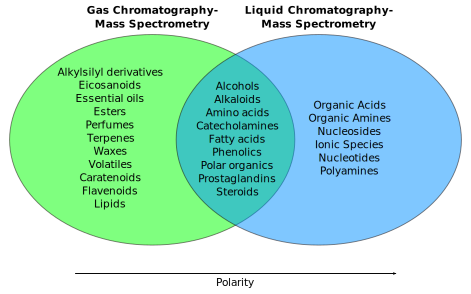
\includegraphics{separation_method.pdf}
    \caption[Compounds by MS Separation Method]{Groups of metabolites by which separation method is best 
    suited for their analysis. Figure redrawn from \url{https://www.agilent.com/cs/library/selectionguide/Public/5989-6328EN.pdf}}
\end{figure}


Mass spectrometry works on the principle that a charged particle moving through an electromagnetic field
is subject to the following two laws: the Lorentz force law (\cref{eq:lfl}) and Newton's second law of motion (\cref{eq:nsl})

\[ F = Q(E + v \times B)\]
\[ F = ma = m\frac{dv}{dt}\]
where \(F\) is the force applied to the ion, \(m\) is the mass, \(a\) the acceleration, \(Q\) the electric charge,
\(E\) the electric field and \(v\times B\) the cross product of the ion's velocity and magnetic flux density. 

Therefore, by combining these two identities:
\[(\frac{m}{Q}) a = E + v \times B\]


\(m/z\) denotes dimensionless quantityy from dividing the mass number of the ion by its charge number.


Mass spectrometry involves 4 components with numerous options and alternative methods for each
optimised for different analytes:
\begin{itemize}
    \item Sample introduction
    \item Ion source
    \item Mass analyser
    \item Mass detector 
\end{itemize}

As mass analysers are only capable of analysing charged ions in a gaseous phase it is necessary to volatilise 
and charge analytes during sample introduction and ionisation respectively. 

While samples can be directly introducted and vaporised using heat or similar, typically most metabolomic
analyses involve the chromatographic separation of samples using either liquid (LC) or gas (GC) chromatography.








\subsubsection{Targeted metabolomics}

There are both targeted and untargeted metabolic analyses that focus on a known set of metabolites such as
amino acids or a global metabolic profile respectively. 





\subsubsection{Untargeted metabolomics}








%gc: Alina dislikes this figure, hard to read
\begin{figure}
    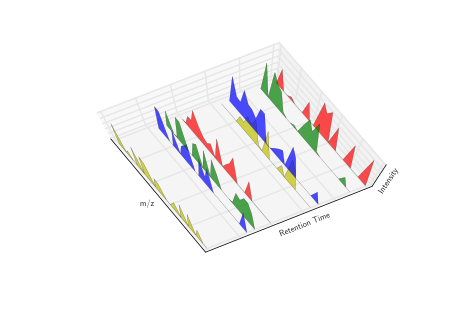
\includegraphics[width=\textwidth]{mass_spec.pdf}
    \caption[Mass Spectrometry Data]{Visualisation of Mass Spectrometry data when coupled with chromatographic techniques.
        The X axis represents the \(m/z\) ratio of an ion, the Y axis the retention time within the chromatographic
    separation method (GC, HPLC etc.) and Z the intensity detected at a given m/z}
    \label{fig:mass_spec}
\end{figure}






These are nuclear magnetic resonance (NMR) spectroscopy, mass spectrometry (MS), 
light (usually infrared (IR) or ultraviolet (UV)) spectroscopy \citep{Kafsack2010}.







There are 3 key techniques used




Evaluating the global metabolic profile (i.e. the presence and absence of 
substrates, products and cofactors) 



It is possible to directly analyse samples using 





By either qualtitatively characterising the presence and absence of various
metabolites under varyin





First commercially available platform was the Vickers ``MS-2'' in 1948





One of the key issues with ``-omic'' platforms is the number of biological replicates 
tends to be far smaller than the number of parameters/metabolites/transcripts being
studied. 


Experimental design: 




Reporting standards \citep{Goodacre2007}

- experimental design



\section{Machine Learning and Statistical Pattern Recognition}

Machine learning is a field of computer science 
devoted to the challenge of developing and applying algorithms capable of 
automatically inferring and utilising patterns in data \citep{Murphy2012}.
A commonly used formal definition of machine learning:
``A computer is said to learn from experience E with respect to some class of tasks 
T and performance measure P, if its performance at tasks T, as measured by P, improves 
with experience E.'' \citep{Mitchell1997} %gc: full stop after citation?
ML encompasses techniques and methods from various areas including statistics,
pattern recognition, optimisation/control engineering, neuroscience and artificial intelligence. %gc: is pattern recognition an area?
Applications range in complexity from simple linear regression to deep convoluted neural networks %gc: convoluted -> convolutional
with millions of free parameters running on dedicated super-computers \citep{Wu2014} 
which are capable of beating human-performance on complex image classification tasks 
(e.g. IMAGENET \citep{Berg2014,He2015}).

Typically, we seek to set the parameters (\theta) of a function in such a way
that another property is minimised.  For example, in linear regression the aim is to find 
parameters of a straight line \(h_{theta}(x) = \theta_{0} + \theta_{1} * x_{1}\) which minimise the distance %gc: Linear regression usually expressed in arbitrary dimensions only includes \theta_{0} as an implied part of the design matrix; see Murphy's derivation
between the line and the data (for example, the sum of squares distance).
This distance/error is calculated using something known as the cost function e.g. \(J(\theta) = \frac{1}{2} \sum^{m}_{i=1} (h_{\theta}(x_{i}) - y_{i})^2\) 
(where \(m\) is the number of \(x, y\) pairs in the dataset for linear regression).
Most algorithms will seek to minimise the value of this cost function \(J(\theta)\) with respect to 
the parameters of the original function \(h_{theta}(x)\).  Typically, this is achieved using a variety of algorithmic optimisation techniques. %gc: theta -> \theta
The most prevalent of these are gradient descent based methods in which the value of \theta is modified %gc: should have \( \)
in the direction of the gradient of the cost function (determined using the partial derivative of \(J\) with respect to \theta: \(\frac{\partial J_{\theta}}{\partial\theta}\)). %gc: don't know if that's necessarily true, linear regression is your most recent example and it has a closed form minimisation


In an ideal world, the best machine learning model trained using our data will generalise well for novel data generated from the same underlying process
which generated the training data.  This is known as generalisability and it plays into the concept of `fit'.  A model that minimises %gc: is generalisability really a word?
its particular cost function on the training dataset has been fit to that dataset, however, it is possible to for the model to fit the training
data in such a way that it has low error on the training data but performs incredibly poorly when applied to new data from the same process.
This is typically the case when a model has overfit the data.  The classic example of this is fitting a line to a set of points using a %gc: more that the situation where this happens is called overfitting. For reference, overfitting is performing worse on the test set than the training set, and underfitting is performing less than perfect on the training set.
high degree polynomial.  This polynomial will perfectly pass through all the points but is likely to be a worse predictor for the value %gc: why are you describing this example with words, just reference figure 1.3.1?
of some new data than a much simpler model that while it fits the original training data, may not fit quite as well.  Likewise, a model that is misspecified
or cannot fit the training data well e.g. the training data follows a non-linear distribution but the model is linear, is known as underfitted.
Underfitted models will perform poorly on both the training and test data.  However, it isn't particularly useful to only discover
how useful your model is likely to be on the test data therefore almost all machine learning analyses will use the principal of cross-validation. %gc: will use or just use?
Cross-validation is the partitioning of the training dataset to create a validation dataset which can be used as a proxy test set.

Unfortunately, no single model will perform best for all tasks (to paraphrase and simplify Wolpert and McCreedy's ``No Free Lunch Theorem'' \citep{Wolpert1996}),
there are no shortcuts in machine learning (and many other areas) or optimisation.  Therefore, testing different models (and hyperparameter values) using
cross-validation is key to generating a useful model.  Another important way to prevent overfitting is to introduce regularisation in the cost function, in other
words a term which penalises model complexity. %gc: Occam's razor? But then you'll have to discuss probabilistic models.

\begin{figure}[h]
    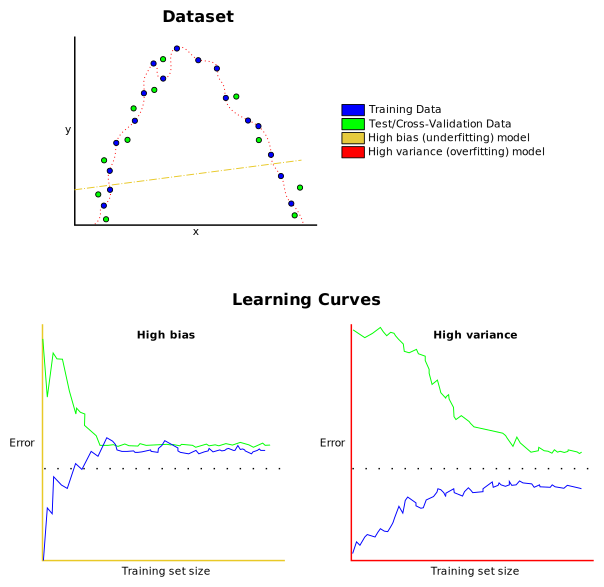
\includegraphics[width=\textwidth]{fitting.pdf}
    \caption[Explanation of Learning Curves and Fitting]{Plot showing a high bias (underfit) model in yellow and a high variance (overfit) model in yellow.
        Below are learning curves corresponding to each of these respectively.
        Learning curves show the effect of different training set sizes on the training and test error of misspecified models.
        Overfitted models show a large gap between test and training errors, they fit to the training data well but don't generalise
        to new data (i.e. test data).
        Underfit models show a very high training error and little difference between test and training data as the model is too simple
        to fit the training data at all.
    }
    \label{fig:fitting}
\end{figure}


%Machine learning can be split into 3 basic components: representation (the form of the model e.g. and input) in which 
%evaluation (cost functions) and optimisation (gradient descent) \citep{Domingos2012}

%Similar to statistics in general, approaches can be parametric or non-parametric in machine learning and can
%be easily distinguished by the change in numbers of parameters are training set size increases.
%For parametric approaches the number of parameters are fixed and finite e.g. when fitting a gaussian distribution
%to a dataset the only parameters are mean and variance of the distribution no matter how many data points are used.
%Non-parametric models on the other hand have an increasing number of parameters as the training set
%increases in size e.g. Dirichlet processes.  Typically, parametric models are faster but are less flexible as
%they make more assumptions about the dataset, whereas non-parametric approaches can be computationally infeasible
%for large datasets \citep{Bishop2006}.
%\section{Fitting}
%``Curse of dimensionality'': as the number of input/feature dimensions increase any training dataset
%will become increasingly sparse.  Parametric models are one solution to this.


Machine learning is typically divided into 2 main subsets depending on the nature of the dataset involved: 
supervised learning (e.g. classification and regression) and unsupervised learning (e.g. clustering,
density estimation and dimensionality reduction).
There are also approaches that blend features of both supervised and unsupervised learning known as semi-supervised
learning as well as an alternative idea known as reinforcement learning built on the premise of the psychology
of behaviour and the indirect reward of trial and error approaches \citep{Bishop2006}.



\subsection{Supervised Learning}

In supervised (also referred to as predictive) learning the principal aim is 
to learn a mapping between inputs/features \(x\) and outputs/response \(y\) from a set of 
inputs and their corresponding expected output.  This is known as the training set 
i.e. \(\mathcal{D} = {(x_{i}, y_{i}) \forall i \in N}\) where \(N\) is 
the cardinality (size) of the training set \citep{Murphy2012}.  
A supervised learning algorithm thus seeks to approximate \(y=f(x)\) where \(f\) is an unknown 
function. This estimated function \(\hat{y} = \hat{f}(x)\) (see \ref{eq:sup}) would then generally
be applied to new data known as the test data for which the expected outputs are not known (i.e. 
\(x_{i} \not \in \mathcal{D}\)).

\[
    \begin{bmatrix}
        x_{0,0} & \cdots & x_{0,j}\\
        \vdots & \ddots & \vdots \\
        x_{i,0} & \cdots & x_{i,j}\\
    \end{bmatrix} \overset{\hat{f}}{\rightarrow} \begin{bmatrix}
        y_{0} \\
        \vdots \\
        y_{i} \\
    \end{bmatrix}
    \label{eq:sup}
\]

Supervised learning is further subdivided into two approaches depending on the nature of the expected
outputs: classification and regression\footnote{It is worth noting that the somewhat confusingly named
    ``logistic regression'' is typically a form of classification}.

In regression the desired outputs are real-valued (or ordinal) i.e. \(y_{i} \in \mathbb{R}\) and we seek to
estimate a particular output quantity for a specific input.
The simplest example of this would be the 2-dimensional linear regression problem mentioned above in which
we are determining the parameters of a line (gradient/weight and intercept/bias) which best fits the training 
dataset (\(\mathcal{D}\)) composed of pairs of \(x\) and \(y\) values.  Once this line has been found we 
can use it to predict the value of \(\hat{y_{i}}\) for data in the test set \(x_{i} \not \in \mathcal{D}\).


On the other hand, in classification the expected outputs are 
categorical or nominal variables such as class labels like ``host'' and ``endosymbiont'' 
(\(y_{i} \in {host, endosymbiont, ... C}\)).  These classifications can be binary (two possible outputs i.e. 
\(y={0,1}\)), multiclass (\(\left\vert{{y}}\right\vert > 2\)),
or multilabel (similar to multiclass but outputs aren't mutually exclusive, i.e. an input have multiple labels
) \citep{Murphy2012}. 

Supervised learning algorithms can also be either probabilistic or non-probabilistic and generative or 
discriminative.
Probabilistic functions will return a probability distribution associated with possible class labels or
regression values whereas non-probabilistic approaches will only return the most likely class label or value.
Continuing 
Generative algorithms, such as Naive Bayes, seek to model the process by which the output data was generated %gc: I thought Naive Bayes isn't a good example of a generative model, but Michael Jordan disagrees so there you go (restricted Boltzmann machines would be more fun)
from the input i.e. learn the joint probability \(p(x,y)\) and make predictions on that basis via Baye's Theorem (see \ref{eq:bayes}) %gc: full stop

\[
    p(x,y) = p(x|y)p(x) = p(y|x)p(y) %gc: should be p(x|y)p(y) and p(y|x)p(y), see https://en.wikipedia.org/wiki/Chain_rule_(probability)
    p(y|x) = \frac{p(x,y)}{p(y)} %gc: I think you meant to split this into multiple equations, it's not all equal
    p(y|x) = \frac{p(x|y)p(y)}{p(x)}
    \label{eq:bayes}
\]

Whereas, discriminative classifiers, such as logistic regression/linear classifiers,
model the posterior probability \(p(y|x)\) directly or just learn mappings in the case of non-probabilistic approaches. %gc: this is usually called the likelihood rather than the posterior, because it would have parameters in the bayesian case, so posterior would be p(w|Y,X) (where Y and X are the whole dataset) and posterior predictive would be p(y*|x*,Y,X) after marginalising w
In other words, for classification problems a generative model would determine the statistical distribution of 
individual classes whereas discriminative models would just determine the boundaries between them.
Generative models often perform better on small training sets by preventing overfitting with discriminative
classifiers performing better as the training set grows \citep{Ng2002}. %gc: not going to argue with Ng and Jordan

\subsubsection{Support Vector Machines}

Support Vector Machines (SVMs) are a type of sparse kernel maximum-margin supervised classification algorithm.
With the innovation of the kernel trick in 1992 \citep{Boser1992} and soft-margins in 1993 (not published until \citep{Cortes1995}) SVMs have been 
among the most successfully applied classification algorithms \citep{Fernandez-Delgado2014}.
Only relatively recently have they begun to lose ground to the deep-learning methods such as deep-convolutional neural networks (e.g. LeNet \citep{LeCunn1998}) exemplified %gc: no dash in deep convolutional or deep learning. Dunno about referencing LeNet as recent, it's old. Recent innovations made it competitive I guess?
by the defeat of SVMs by the LeNet on the MNIST digit recognition dataset \citep{Hinton2006,Bengio2007} \citep{Bengio2013} %gc: full stop

The goal of SVMs is to learn a hyperplane which separates two sets of labels in the dataset. Note, for multiclass classification a series of one-vs-all
classifiers are typically trained (that is for \(K\) classes, \(K\) SVMs are trained each classifying between a label \(k\) and all other labels).
However, not all possible hyperplanes that could separate the labels will necessarily generalise well to novel data (and this generalisation
is the ultimate goal of supervised learning).  Therefore, it is necessary to determine a way to select the hyperplane which should generalise best and to do
this in a manner that will be relatively efficient especially with high dimension datasets.  This optimal hyperplane for separable classes can be demonstrated to be
the hyperplane which maximise the margin between the two classes \citep{vapnik1982estimation} in other words, the optimal boundary is the one that has the largest %gc: maximise -> maximises, full stop then "In other words..."
possible distance from each class (while still separating them).  Conceptually, the positioning of this boundary is only dependent
on the relatively small subset of the training data \(\mathcal{D}\) that is near the boundary and it would be inefficient to consider all points when
placing the decision boundary.  For this reason, SVMs can define the decision boundary in terms of the namesake support vectors and can reformulate
their cost function in a more efficient constrained way.

\begin{figure}[h]
    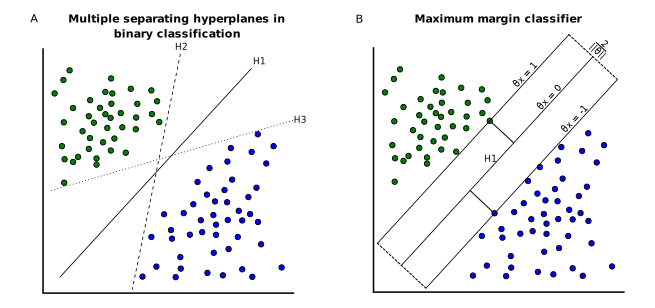
\includegraphics[width=\textwidth]{margin.pdf}
    \caption[SVM Decision Boundaries]{A: Demonstration of 3 valid decision boundaries in a 2D classification problem, B: The optimal boundary (H2) is that which maximises
        the separation of different classes.  This optimal boundary can be defined in terms of support vectors.  The bias/intercept has been 
    folded into \(\theta\) directly.}
    \label{fig:margin}
\end{figure}

A naive formulation of this problem is simple specifically we are trying to find a linear model \(f(x) = \theta_{0} + \theta^{T}x\) which can be simplified 
to \(f(x) = \theta * x \) if we assume that the first element of \(x\) is fixed to \(1\). We thus want to minimise \(J\) in terms of \(\theta\) to find
the largest margin that correctly labels all the training data (in other words is constrained).  Fortunately, due to geometry the margin is property of
the norm of \(\theta\) i.e. \(||\theta||\) but we use \(\frac{1}{2} ||\theta||^{2}\) for mathematical convenience.

\[argmin_{\theta} J(\theta) = \frac{1}{2} ||\theta||^{2} s.t. y_{i}(\theta x_{i}) \geq 1 \forall i\]

In reality, this cost function would be converted to a constrained optimisation problem using Lagrange multipliers and reformulated using the Lagrangian dual form. 


The 2nd major enhancement of SVMs is that of soft-margins \citep{Cortes1995}. Soft-margins are a way of allowing a degree of misclassification
if doing so would increase the size of the margin that can be generated.  Specifically, a user defined penalty constant \(C\) is specified and 
added to the cost function penalising the degree of misclassification \(\xi\), e.g.:

\[argmin_{theta} J(\theta) = \frac{1}{2} ||\theta||^{2}  + C \sum^{n}_{i=1} \xi_{i} s.t. y_{i}(\theta x_{i}) \geq 1 - \xi_{i} \forall i\] %gc: theta -> \theta

This can improve robustness to outlier data and generally improve generalisability by keeping the margin as large as possible.

\begin{figure}[h]
    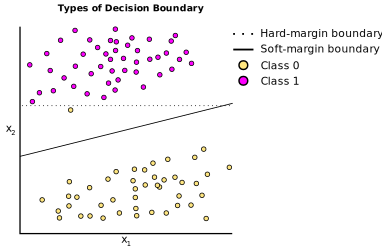
\includegraphics[width=\textwidth]{boundary.pdf}
    \caption[Soft-Margin Classifiers]{Demonstration of the utility of a soft-decision boundary to improve the overall
    fit of a decision boundary by allowing a degree of misclassification during training}
    \label{fig:boundary}
\end{figure}

Finally, the 3rd major advantage of SVMs is that despite nominally being linear classifiers they can effectively classify data which 
is not linearly separable in the input dimensions using the kernel trick.  Conceptually, a kernel function is used to transform %gc: No citation for the kernel trick?
which transforms data from the input dimensions to a higher dimensional space in which the data is linearly separable.
These transformed feature spaces can have incredibly high number of dimensions (in the case of popular kernels like radial basis
function, an infinite number of dimensions).  Explicitly transforming data in this way would be computationally intensive
so instead the ``kernel trick'' is used, where instead of explicitly transforming all the data into the feature space
it is done implicitly by computing the inner product of all pairs data points transformed.  This is a lot more efficient
and precludes the computationally intensive step of converting the data into the new, potentially infinite, co-ordinate space.
Radial basis function (RBF) kernel is an example \(K(x_{i}, x_{j}) = exp ( - \frac{||x_{i} - x_{j}||^{2}}{2\sigma^{2}})\) kernel.
Even with the kernel trick, operations on every pair of points can become infeasible for large datasets due to the combinatorial
explosion in necessary operations as the dataset increases in size.  However, in the same way that the decision boundary parameters 
are determined using only a subset of the training data (i.e. the support vectors) the kernel trick only needs
evaluated on a subset of points near the decision boundary.  This is the reason SVMs are sometimes
referred to as sparse kernel methods.

\begin{figure}[h]
    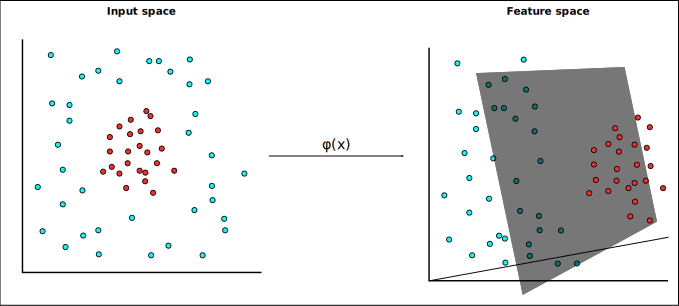
\includegraphics[width=\textwidth]{kernel.pdf}
    \caption[Kernel Trick]{A kernel transform can allow SVM to produce non-linear classification boundaries by mapping
        the data to a higher dimensional space in which they are linearly separable. This is known as the kernel
        trick and the key to its efficiency in SVM is that it is only evaluated for those sets of points near the 
    decision boundary}
    \label{fig:kernel}
\end{figure}



The advantages of SVM is that they are somewhat resistant to the curse of dimensionality i.e. they are effective with large numbers of features
even if the number of features is greater than the size of the training set.%gc: you should probably back this up, or don't make the claim
By using support vectors, the kernel trick, and Lagrange bound optimisation 
they are relatively fast and memory efficient to train and as classification only depends on the location of the decision boundary very fast to test.
Additionally, in simple form finding the hyperplane of an SVM is a true convex optimisation therefore is guaranteed to always find the global optimum (this %gc: an SVM -> a SVM, true convex optimisation *problem*
guarantee does break with more complex kernels and soft-margins).  
The major disadvantage is not natively generating probabilistic output (i.e. attaching a probability to a certain classification).  However, this can be achieved
using methods like Platt Scaling or the related Relevance Vector Machine algorithm.   The other disadvantage is that hyper-parameters such as the misclassification %gc: citations for those methods? Also, there is a probabilistic derivation of support vector machines on p.505 of Murphy's textbook, section 14.5.5
penalty for soft-margins (\(C\)) and kernel choice (and its parameters) need chosen, typically this is solved by training using a grid-search of permutations
of these parameter settings and selecting the best model via cross-validation.


\subsection{Unsupervised Learning}

The other main form of machine learning is that of unsupervised or descriptive learning.
In which the training dataset has no provided output labels (y) i.e. 
\(\mathcal{D} = {x_{i} \forall i \in N}\) (where again N is the cardinality of 
this training dataset). In other words, we just have our dataset and have no additional information.
This is slightly more difficult problem as it lacks an obvious error metric like supervised learning 
(i.e. difference between actual output and expected output) but is important and useful tool to
try to discover patterns in datasets.

There are two major groups of unsupervised learning algorithms, the first of which is clustering algorithms
such as K-means that seeks to partition a dataset into a set of groups (see \ref{fig:kmeans} for more details).
The other major group of unsupervised algorithms are those used for visualisation and/or
dimensionality reduction.  Dimensionality reduction is a way of projecting a multidimensional
dataset into a lower number of dimensions in a way that still corresponds to
``shape'' of the data in the original number of dimensions.  

Formally, dimensionality reduction seeks to take a set of data (\(\mathcal{D}\)) and convert it
to a lower dimension form \(\mathcal{Y}\) known as a map \(\mathcal{Y} = {y_{i} \forall i \in N}\) 
with each individual \(x_{i}\) in \(\mathcal{D}\) represented by a corresponding map point \(y_{i}\). It
also seeks to do this in a way that maintains as much of the structure found in the original data 
as is possible \citep{Maaten2008} therefore, if two data points are similar in the original dimensions
they should still be similar in the map \(\mathcal{Y}\) (and the inverse).
Some dimensionality reduction approaches are well known in biology, specifically: principal component analysis (PCA) 
\citep{hotelling1933analysis} and multidimensional scaling (MDS) \citep{Torgerson1952} which both aim to identify
hidden features within the dataset that can explain a high degree of the variation.  


As ever different methodologies have a range of pros and cons, with
some better at preserving global structure (e.g. isomap) and others local data structures (e.g. local linear embedding) and so on.
One of the most recent innovations in this area is that of t-distributed stochastic neighbour-embedding
(t-SNE) in which the similarity of data points in the input space is modelled as pairwise probabilities 
using Gaussian distributions.
These probabilities are then translated into positions in the map \(\mathcal{Y}\) and similarities re-calculated
using Student's t-distributions.  The position and variance of these points and distributions respectively
is then optimised by minimising the difference between the similarity probabilities in the input space
and on the map \citep{Maaten2008}. %gc: this is probably right, but my understanding of t-sne isn't great

\subsubsection{K-means}

K-means clustering is a non-probabilistic unsupervised learning 
method in which we seek to partition data points in multidimensional space into 
K clusters. It is often used to initialise Gaussian mixture models.

Specifically, given a set of \(N\) observations \(X = {x_{1},...,x_{N}}\) 
of \(\mathcal{D}\) dimensions partition each point \((x_{n})\) into K clusters %gc: unfinished?

A cluster can be intuitively considered as a group of observations/points which are 
``closer'' to one another than to other observations and the k-th cluster can 
defined by a \(\mathcal{D}\) dimensional vector \(\mu_{k}, where k=1,..,K\) for all clusters.
This vector represents the current ``prototype'' centroid of cluster. 

So, with k-means clustering we actually seek the set of K cluster centroids \({\mu_{k}}\) 
which minimise the sum of squares distances of each data point from its closest cluster centroid.
\citep{Bishop2006}

If we define a 1-of-K coding scheme with \(r_{nk} \in {0,1}\) as a binary variable that is 1 when \(x_{n}\) has been
assigned to cluster \(k\) (with centroid \(\mu_{k}\)) and 0 otherwise then we can define an objective cost function (\(J\)) 
that represents the sum of squares distances of each data point \(x_{n}\) from its assigned cluster centroid \(\mu_{k}\).

\[ 
    J = \sum_{n=1}^{N}\sum_{k=1}^{K} = r_{nk} \|x_{n} - \mu_{k}\|^{2} %gc: why is there an equals sign in here?
    \label{eq:kmeans_cost}
\]

Therefore, the goal of k-means clustering is to find values for \({r_{nk}}\) and \({\mu_{k}}\) that minimise this linear 
function \ref{eq:kmeans_cost}.
\citep{Bishop2006}


The standard algorithm proceeds in two alternating steps following the initialisation of \(\mu_{k}\) with starting
cluster centroid locations \citep{Forgy1965,Lloyd1982}:
\begin{enumerate}
    \item \(argmin_{r_{nk}} J\) i.e. minimise \ref{eq:kmeans_cost} w.r.t the assignment of points to clusters while keeping
        the cluster centroids fixed.
    \item \(argmin_{\mu_{k}} J\) i.e. minimise \ref{eq:kmeans_cost} w.r.t the position of the cluster centroids while keeping
        the assignment of points to centroids fixed.
\end{enumerate}

Step 1 roughly corresponds to the expectation step in the expectation-maximisation (EM) algorithm and is trivially achieved by 
assigning each point to the cluster represented by the nearest centroid or formally:
\[
    r_{nk} = 
    \begin{cases}
        1,& \text{if} k=argmin_{j} \|x_{n} - \mu_{j}\|^{2}\\
        0,& \text{otherwise}
    \end{cases}
\]

Step 2 roughly corresponds to the maximisation step in EM is can be determined by taking the partial derivative of \(J\) w.r.t 
\(\mu_{k}\) setting it to 0 and solving for \(\mu_{k}\):
\[
    \frac{\partial J}{\partial \mu_{k}} = 2 \sum_{n=1}^{N} r_{nk} (x_{n} - \mu_{k}) %gc: this should be split over multiple lines?
    0 = 2 \sum_{n=1}^{N} r_{nk} (x_{n} - \mu_{k})
    \mu_{k} = \frac{\sum_{n} r_{nk}x_{n}}{\sum_{n} r_{nk}}
\]

In other words set \(\mu_{k}\) to the mean of all data points \(x_{n}\) assigned to cluster \(k\) thus k-means \citep{Bishop2006}

These two steps are repeated until a specified maximum number of iterations are reached or no points change cluster assignment during
step 1.

\(J\) \ref{eq:kmeans_cost} will converge but is liable to get stuck in a local rather than global minimum. %gc: J in eq. 1.3.2?

K-means has many modifications and improvements such as refining the initialisation of the clusters by 
the Bradley-Fayyad method (clustering random samples of the dataset and then k-means clustering the resulting clusters) \citep{Bradley1998} 
or over-clustering (running more than k-means clustering with more than the specified number of clusters and merging clusters at the end
to generate the correct number of clusters). One of the most recent and promising improvements is that of ``ying-yang'' k-means
clustering which gains a moderate speed-up over the conventional algorithm by minimising the number of distance calculation required.
This is achieved by creating upper and lower bound distance filters using the triangle inequality (i.e. \(d(a,b) \leq d(a,c) + d(b,c)\) where 
\(d\) is a function that calculates the distance between 2 points) \citep{Ding2015}.



An efficient implementation of the k-means algorithm is available in the MLPACK C++ Machine Learning library \citep{mlpack2013}.
While very efficient and effective, k-means has some limitations, it requires a user specified number of clusters
and therefore diagnostics to check for obvious misspecification in the number clusters.  Information criterion
can be used to determine the optimal number of clusters. %gc: criteria, maybe? I don't know, you read the sentence. I guess this is important because you used it?
Additionally, it is not guaranteed
to discover the global optimal clusters (can converge to local optima).  This can be amortised by running multiple times 
with different initialisations.

\begin{figure}[h]
    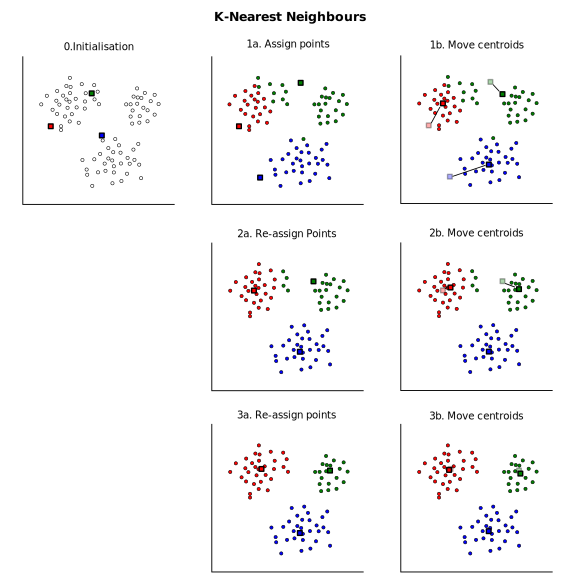
\includegraphics[width=\textwidth]{knn.pdf}
    \caption[K-means Clustering]{Demonstration of the K-means algorithm applying 3 rounds of Expectation-Maximisation to cluster
        a group of 2 dimensional samples.  The 3 cluster centroids (represented by coloured rectangles) 
        are randomly initialised in 0 before undergoing 3 rounds of EM.  
        This involves the successive assignment of samples to their nearest centroids (1a, 2a, 3a) 
and then the movement of the centroids to the center of the points currently assigned to that centroid (1b, 2b, 3b).
Assignment of a given sample to a centroid is indicated by a shared colouring and centroid relocation by
an arrow with a faded version showing the initial location.
}
    \label{fig:knn}
\end{figure}

\section{Phylogenetics}

Phylogenetics is an effective tool (if there is sufficient signal/resolution) 
to investigate the evolutionary ancestry of biological sequence data.
It can be used to identify how closely related a given pair of sequences are, as
well as indicate what the sequence most likely looked like in a shared common
ancestor (ancestral node reconstruction). Phylogenetic methods also allow estimation
of evolutionary processes such as selection pressure,
migration, genome reduction, and horizontal gene transfer.
In the context of endosymbiosis, phylogenetics can be used to determine evolutionary ancestry of 
the genes recovered in a transcriptome and to aid identification of the likely origin 
(host, endosymbiont, contaminant) of these transcripts. Additionally, it can pinpoint
potential horizontal gene transfer events between host and endosymbiont by searching for single 
gene/transcript phylogenies that have an incongruent branching pattern
compared to established species trees.  Finally, it can be used to aid identification of the putative function 
of novel transcripts by comparison to other transcripts of known function 
from databases such as genbank. 


Phylogenetics can be defined as a means of arranging a set of character sequences into an optimal hierarchial
branching tree structure reflecting some measure of relatedness 
between the sequences. Usually, these trees will have variable
branch lengths that are product of a measure of divergence between the connected nodes.

Typically, these sequences take the form of protein or DNA sequences\footnote{
Strictly phylogenetics refers to the study of molecular sequence data although the same methods are applicable to
non-molecular characters such as morphological traits (and occasionally originated in this domain) as well as any
other set of discrete data vectors. It has even been applied to fields such as linguistics \citep{}
} and the measure of relatedness is some proxy for evolutionary distance ranging from simple distance measures 
e.g. Hamming distance (\(D = \sum_{k=0}^{N}|x_{k} - y_{k}|\) for two sequences \(x\) and \(y\) of length \(N\))
to more complicated probabilistic estimations based on observed data.
A character is an element of a sequence such as an individual base or amino acid, homologous 
characters are those in separate sequences that are descended from a common ancestor.  
As they were the first molecular sequences easily available much of the early work in molecular phylogenetics
was conducted using protein sequences e.g. \citep{eck1966atlas,Fitch1967}.

This phylogenetic estimation can be a non-trivial process (especially with more complex
measures of relatedness) as the number of
possible trees rapidly increases with the number of sequences \(N_{trees} = \prod_{x=2}^{N_{taxa}} (2x - 3)\).
However, the key stages in a phylogenetic analysis are that of sequence sampling (selection of
sequences for inclusion in the analysis),  alignment (in which homologous sites in the sampled sequences are aligned with one another),
 masking (in which sites which are evolutionarily informative – can be determined to be homologous 
     but also non-invariant are selected), model selection (in which the best fitting
 evolutionary model is selected or calculated) and finally, phylogenetic reconstruction (in which the tree
 is generated that minimises some measure e.g. most likely tree for probabilistic models or 
 least distance).


%
%There are 4 major sources of error in the generation of phylogenetic trees that 
%can be reduced to greater and lesser extents depending on the methodology used.
%Compositional bias 
%
%
%
%
%Long branch attraction is one of the most famous artefacts, it is the erroneous grouping of long (usually fast evolving)
%branches in a tree as sister groups.  It is caused by 
%
%
%Sequence sampling is important both between taxa and within taxa.
%
%Hidden paralogy is another artefact that can be exacerbated with poor taxon sampling, this occurs when a sequence has
%been duplicated within an ancestral taxa (creating paralogs) but differentially lost in its descendents.  
%If, due to either deletion or poor sampling, the incorrect paralog is incoporated into a phylogeny 
%
%
%Homoplasy - convergent evolution
%Poor taxon sampling that is unrepresentative of the diversity that the phylogenetic tree
%is intended to span 
%




One implication of most current phylogenetic methods is that they implicitly
assume a branching tree structure is the best representative of the evolutionary
process that is being modelled.  However, as the discovered prevalence of
horizontal gene transfer has increased it is becoming that in some cases
a network like structure may in fact be more appropriate.


Most analyses in this PhD are conducted using amino acid sequences.  
DNA is more likely to display a compositional bias, independence of sites
is often severely violated due to the structure of codons (3rd base wobble and so on)
(non-synoynmous mutations more likely to become fixed whereas synonymous mutations are
prone to drift).  Amino acids also have more states so are less susceptible to back mutations
than DNA.  


\subsection{Sequence sampling}
Sequence sampling, the selection and identification of sequences for initial inclusion in a 
phylogenetic analysis, is arguably the most important stage in phylogenetic analysis.
Any biases introduced here will propagate throughout the rest of the analysis. 
While some biases can be mitigated to lesser and greater extents 
by careful application of various methods in the following
stages, there is a degree of fundamental truth in the statement ``garbage in - garbage out''.

The aim of proper taxon sampling is to maximise phylogenetic accuracy and to allow
testing of specific hypotheses. 
Phylogenetic accuracy is usually considered in terms of consistency (as data increases 
    the analysis tends towards the correct tree), efficiency (how quickly does this convergence
occur), and robustness (how sensitive is the phylogeny to violation of assumptions in reconstruction) \citep{Nabhan2012}
Typically, sequence sampling will be conducted from the basis of a single
seed sequence which will be used to query existing databases using alignment 
tools such as BLAST and HMMs (explained in \ref{nextsection}) to attempt to discover %gc: broken cross-ref?
potentially homologous sequences from different organisms.  


The main issues caused by poor taxonomic sampling in molecular phylogenetics are that
of conflicting phylogenetic signals, inadequate rate of evolution to resolve relationships
of interest, and violations of assumptions e.g. expectation of a uniform distribution of traits \citep{Nabhan2012}.


Generally, increased taxon sampling has a strong positive effect on
phylogenetic accuracy \citep{Zwickl2002} %gc: full stop and new sentence?
however, it can also lead to a situation where there are too many sequences to
efficiently reconstruct a phylogeny.  However, care care must also be taken not
to unintentionally bias datasets by removing any sequences that are considered
``problematic'' especially when conflicting phylogenetic signal or model
violations can be biologically informative.  Therefore, it is usually necessary
to include borderline error-generating sequences within a phylogeny initially
and to iteratively remove them and repeat the phylogenetic inference. %gc: two ands in one sentence
Unfortunately, the reduction of the input sequences to a representative subset
by heuristics and/or naive clustering can generate biases of their own. %gc: biases of their own -> new biases
However, tools exist that utilise taxonomic database information to
automatically a subset of specified cardinality of sequences that display the %gc: automatically a subset?
maximium possible taxonomic diversity for that subset size \citep{Zhou2014}.

Another source of bias in sequence sampling is the usually heuristic choice of
outgroup taxa. Most contemporary models of phylogenetic inference only infer
unrooted trees.  Therefore, it is common practice to ``root a tree'' by
selecting a set of sequences from known evolutionarily distance organisms to
form an outgroup. If this outgroup is correctly recovered (monophyletically) %gc: comma?
the root can be placed between it and the other sequences in the phylogeny
\citep{Yang2012}.  However, choice of outgroup can change implications which
may be drawn from a phylogeny regardless of methodology used to infer it
\citep{Milinkovitch1996}.  and care must be taken to ensure the selected %gc: new sentence capitalisation and comma after the and
outgroup doesn't actively distort the accuracy of inference of the rest of the
phylogeny regardless of the issue of root placement \citep{Milinkovitch1998}.

The two principal ways in which putatively homologous sequences are identified
in sequence databases are those based upon Basic Local Alignment Search Tool
(BLAST) and its variants and Hidden-Markov Model based approaches (HMM).  We
seek a way of identifying and aligning homologous sequences in a target
sequence database with our query sequence. %gc: what? does this make sense?

%
%\subsubsection{BLAST}
%
%BLAST, its variants and improvements are the most widely used algorithms currently used to search sequence databases.
%Fundamentally, they are sequence 
%
%Likely homologous sequences can be identified via weak but biologically significant sequence similarities to a
%given query sequence.
%
%
%
%A variation BLAT (Basic Local Alignment Tool)
%
%
%
%
%to identity likely homologous sequences 
%to a given query.
%
%
%
%\subsubsection{HMM}
%
%Hidden Markov models are an established method to probabilistically model
%sequences of data such as a series of events or residues.
%A hidden Markov model consists of a finite number \(N\) of states 
%with transition between states determined at a fixed interval using a 
%transition probability distribution dependent on the previous state.
%This is known as the Markov property: ``the independence of the future from the
%past, given the present''.
%Hidden refers to the fact the true states are a latent process that must
%be inferred indirectly from the observed data.
%For example, if the HMM states are the set of conserved protein domains
%making up a particular query 
%An HMM is specified with a finite symbol alphabet e.g. the set of amino acid residues,
%the number of model states, emission probability for each state that normalise to 1
%over the symbol alphabet and the transition probabilities for each state
%going to any other state (self included) marginalising to 1 over states
%\(K\) symbol alphabet
%
%The 3 benefits of Markov models are: 
%\begin{itemize}
%    \item incorporation of heterogeneous
%sources of information e.g. combining data about codon bias, exon distribution and/or 
%splice-sites with the underlying DNA sequence.
%    \item full probabilistic output instead of an arbitrary score function
%    \item general and extensible i.e. the HMM can be extended to incorporate new sources of information as they are discovered \citep{Eddy2004}
%\end{itemize}
%
%HMMs are used widely in biology especially versatile with sequence data applications such as search for sequences
%annotation.
%They are at the heart of a diverse range of programs, including genefinding, profile searches, multiple sequence alignment and regulatory site identification
%
%Highly sensitive, specificity depends on quality of MSA.
%
%Detection of sequence divergent homologs
%
%
%
%Supertree generate tree for each gene and use heuristic algorithm to combine \citep{Bininda-Emonds2004}, can spot HGT but is inefficient
%
%Supermatrix, concatenation \citep{DeQueiroz2007a} - ignore differences in dynamics between gene, if partitioned then same as supertree
%
%Best approach is supermatrix with a model that incoprotates rate heterogeneity \citep{Ren2009}
%

\subsection{Multiple Sequence Alignment (MSA)}

The goal of MSA is to align sets sequences such that evolutionarily homologous
residues occupy the same column. In other words, any given column in the
alignment theoretically should contain amino acid or nucleotide residues that
derive from the same common ancestor and have evolved in each sequence lineage.
It is also possible that insertion or deletion events have taken place and a %gc: does this make sense? surely if instead of and
particular residue is absent in the ancestral node or a sequence lineage.

This is a non-trivial computational problem which has been proven to have an
NP-complete \footnote{A decision problem for which an answer can be verified in
polynomial time by a non-deterministic turing machine and to and from which %gc: capitalise Turing
any NP-hard problem can be translated \citep{Karp1972}.}
computational complexity \citep{Wang1994}.  Specifically, the optimal alignment
of N sequences has a complexity of \(O(L^{N})\) for \(N\) sequences of length
\( L \)\citep{Sievers2011}.

Due to this complexity, the majority of MSA algorithms implement heuristic
approaches in order to get, if not the optimal solution, but a sufficiently %gc: then instead of but?
good one in a reasonable amount of time. 

Typically, MSA algorithms start by generating the sets of all pairwise
alignments using established pairwise alignment algorithms.  Pairwise alignment
algorithms are almost all based upon a pair of ``Ur-algorithms'' with different
goals: Needleman-Wunsch, a global alignment algorithms (which attempt to %gc: attempts
maximise alignment quality over entire sequence lengths) \citep{Needleman1970}
and Smith-Waterman, a local alignment algorithms (which are optimised towards %gc: algorithm, which is
producing high quality alignments in sub-strings) \citep{Smith1981}.  While
early, MSA algorithms were typically largely derived from Needleman-Wunsch most %gc: new sentence?
modern algorithms seek to combine optimisation of local and global alignments.
The distances used in these pairwise alignments will typically be ``scored''
based upon which matches or alignments are more frequent substituions (e.g.
Leucine and its isomer Isoleucine or Adenine to its fellow purine base Guanine
(transition)) are positively scored and gaps (extension of a gap is typically
less penalised than creating a gap) or unlikely changes (e.g. the transversion %gc: this sentence is hard to read
of Adenine to Cytosine or Glutamine to Cysteine) penalised.  This will 
generally be codified in a substitution matrix e.g. the PAM
\citep{Dayhoff1978}, BLOSUM \citep{Henikoff1992} amino acid matrices and their
numerous subsequent derivations and improvements. 

The mostly widely heuristic used to go from these series of pair-wise
alignments to a useful MSA is that of progressive-alignment \citep{Feng1987}
(implemented in tools such as CLUSTAL W \citep{Thompson1994}) in which the %gc: comma or semicolon
pairwise alignment scores are built into a distance matrix summarising the
relative divergence of each pair of sequences. From this matrix a
``guide-tree'' is generated using simple neighbour-joining methods (in which a
tree is built by recursively clustering the least dissimilar sequences
\citep{Saitou1987}).  Sequences are then progressively aligned using their
branching order within this guide-tree \citep{Thompson1994}..  This drastically
reduces the \(O(L^{N})\) complexity to approximately \(O(N^{2})\)
\citep{Sievers2011}. While there have been various improvements and alternative
approaches created such as merging both local and global alignment
\citep{Notredame2000}, rapid identification of homologous regions using Fast
Fourier Transforms \citep{Katoh2002}, iterative refinement of alignments
\citep{Edgar2004a} and use of Hidden-Markov Models \citep{Eddy1995} %gc: full stop

There have been compelling arguments as early as 1991 that MSA in isolation
from phylogenetic inference is inherently flawed as the consideration of
evolutionary processes (only really done during phylogenetic inference) is key
in the objective weighting and assessment of potential alignments
\citep{Thorne1991}. Therefore, the phylogeny and MSA should be jointly
inferred \citep{Thorne1991,Redelings2005,Bouchard-Cote2013} This approach also %gc: full stop
minimises the risk of conscious or subconscious researcher bias towards
alignments and subsequent phylogenies that support their pre-conceived ideas.
This approach has been attempted using interesting probabilistic programming
approaches i.e. BALI-phy \citep{Suchard2006}, however, it is still far too slow %gc: another comma before i.e. could new sentence after
a process to infer phylogenies in this manner on large or even moderate
datasets.  Therefore, for now, independent MSA estimation is here to stay, at
least until computational resources and algorithmic development has continued
until these more theoretically satisfying approaches become feasible.  

Therefore, throughout this thesis, two progressive/iterative alignment tools
will be used: Kalign2 \citep{Lassmann2005,Lassmann2009} for high-throughput
analyses and iteratively refined MAFFT7 \citep{Katoh2002,Katoh2005,Katoh2013}
for individual accuracy critical phylogenetic analyses.  Kalign is a very
high-speed and relatively accurate \citep{Thompson2011} progessive alignment
tool that uses an efficient and fast Wu-Manber approximate string-matching
algorithm to calculate sequence distances \citep{Lassmann2005}.  MAFFT, with
iterative refinement, is a relatively slow but highly accurate MSA alignment
method \citep{Thompson2011} that incorporates all pairwise alignment
information when refining instead of using heuristics to approximate pairwise
sequence differences like most approaches.

\subsection{Masking}

Unfortunately, MSA is far from perfect, especially with the faster algorithms
necessary for larger datasets and higher throughput.  Therefore, it is often
necessary to trim alignments to manually fix any obviously misaligned residues,
and remove any ambiguously aligned or absent sites.  This has been demonstrated
to improve phylogenetic accuracy \citep{Talavera2007}.

However, manual masking can also be a major source of researcher-bias as well
as a painstaking process. For this reason, there are tools that attempt to
automate this process. They typically score each column independently with
criteria including number of absent character states, how similar/variable the
character is and if there are multiple putative alignments - how likely is that
column to be found in multiple different MSAs. These criteria can then be used
to mask out certain columns based on certain thresholds and trade-offs between
the length of the alignment and inclusion of low-scoring columns. TrimAL is an
example of a tool that automates the masking process using this sort of
methodology \citep{Capella-Gutierrez2009}.  

Similarly to MSA, for high-throughput analyses I will use TrimAL whereas for
individual accuracy critical analyses masking will be done manually using the
graphical tool Seaview \citep{Gouy2010}.

\subsection{Substitution model selection}

While the simplest means of phylogenetic inference - parsimony i.e. finding the
tree that requires the fewest sequence changes does not require any explicit %gc: another dash after changes, if you're doing dash parentheses (you are)
model of sequence evolution, all other means of phylogenetic inference do
\citep{Le2008}.

A substitution model is in its simplest sense the same as the PAM and BLOSUM
matrices used in pairwise and MSA. They are a means of scoring and weighting
the significance of different character changes, is an A to a G a more %gc: is it? maybe just say it is?
evolutionarily rare state change than an A to a T for example.

Substitution models typically assume neutrality, independence and finite sites.
With the probability of substitution rates having an independently identical %gc: subsitution rates assuming a distribution that is independent and identically distributed (and remember a full stop after)
distribution (i.i.d) \citep{Hasegawa1985} This measure of distance can be naive
models where rates of change between character states and the frequency of each
state is equal (e.g. \(p(x \rightarrow y) \forall x \forall y \in {G,C,T,A}
\text{where} x\neq y\) \citep{jukes1969evolution}) to models fully
parameterised in terms of character frequency and rates of change by the masked
alignment (e.g. the generalised time-reversible (GTR) model \citep{Tavare1986}) %gc: full stop
%
%\begin{figure}
%    \[
%    Q=\begin{pmatrix}
%        \.             & \alpha\pi_{C}   & \beta\pi_{A}    & \gamma\pi_{G} \\ 
%        \alpha\pi_{T} & \.               & \delta\pi_{A}   & \epsilon\pi_{G} \\ 
%        \beta\pi_{T}  & \delta\pi_{C}   & \.               & \zeta\pi_{G} \\ 
%        \gamma\pi_{T} & \epsilon\pi_{C} & \zeta\pi_{A}    & \. \\
%    \end{pmatrix} 
%
%    Q_{ii} = - \sum_{\{j | j \neq i\}} Q_{ij}\\
%
%    \Pi = (\pi_{G}, \pi_{T}, \pi_{C}, \pi_{A})\\
%
%    \Pi * Q = 0 \\
%
%    \alpha = p(T \leftrightarrow C)\\
%
%    \beta = p(A \leftrightarrow T)\\
%
%    \gamma = p(G \leftrightarrow T)\\
%
%    \delta = p(C \leftrightarrow A)\\
%
%    \epsilon = p(G \leftrightarrow C)\\
%
%    \zeta = p(A \leftrightarrow G)
%    \]
%        \caption{Generalised time-reversible model for DNA sequence evolution under a reversible homogeneous Markov process where \(\Pi\) is the 
%        frequency of each state and \(\alpha\) through \(\zeta\) are substitution rates \citep{Tavare1986,Yang1994}.  All other Markov process models
%    of sequence evolution are special cases of GTR.   Time-reversibility refers to the fact that \(\pi_{i}Q_{ij} = \pi_{j}Q_{ji}\) therefore
%   the direction of state changes is irrelevant}
%        \label{eq:gtr}
%\end{figure}
%
While models like GTR can feasibly be fully parameterised with DNA sequence
data due to DNA's relatively few character states it is usually necessary to 
use empirically-defined models for amino acid datasets.  These are substitution
matrices that have been determined using the empirically observed substitution
rates for various amino acids changes in many large MSAs \citep{Le2008}.


Unfortunately, a single substitution model will rarely hold true over an entire
alignment with the rate of evolution varying both across and within sites
(heterogeneity and heterotachy). The frequency of character states also
frequently changes across a phylogeny.  It is important to control for these
phenomena, because, as mentioned earlier, violation of model assumptions can
decrease phylogenetic accuracy.


The most frequent violation that is controlled for is allowing the rate of
substitution to vary across sites by using a \(\Gamma\) distribution \(Var =
\frac{\alpha}{\beta^{2}}, \mu = \frac{\alpha}{\beta}\) with a given shape
\(\alpha\) and trivial scale factor \(\beta\) depending on the dataset to scale
rates at each site.  For datasets that have a high degree of rate heterogeneity
a low valued \(\alpha\) produces a broad distribution of rates, whereas a high
value will generate a narrow distribution for datasets with low rate
heterogeneity \citep{Yang1993}.  For reasons of computational efficiency
\(\Gamma\) is typically approximated as a discrete distribution of 4 to 8
categories of equal probability \citep{Yang1994a}.  A more limited version of
this is the invariant sites model in which sites are divided into 2 classes,
one considered invariable while the other has normal substitution rates
applied\footnote{ This can also be used with \(\Gamma\) and is approximately
equivalent to the addition of another discrete \(\Gamma\)
category}\citep{Hasegawa1985}.  %gc: need a full stop in the footnote as well



Unfortunately, these models still assume other model parameters namely the
equilibrium frequencies and relative rates are the same across sites (but just
scaled).  However, some models have been proposed with multiple rate matrices
\citep{Lartillot2004} and state frequency can be defined at each site %gc: state frequencies?
\citep{Bruno1996} but needs lots of taxa \citep{Lartillot2004} An alternative %gc: full stop
to this is the CAT model which a mixture model mixture model with K classes
each containing a different state frequency.  If \(K=N\) then this is the same
as Bruno's model however, generally \(K < N\).  A probabilistic process known
as a Dirichlet Process Prior is used to assign columns to various state
frequency classes and simultaneously determines the optimal value of \(K\)
during this process \citep{Lartillot2004}.  An alternative to this approach is
explicitly partitioning a masked alignment and generating a model and state
frequencies for each partition, some consider this equivalent to a CAT model
depending akin to preferences for fixed-effects vs random-effects models
\citep{Yang2012}.  However, personally, automated partitioning using a
Dirichlet process has the advantage of not requiring arbitrary user-defined
partitions, which could be a source of bias.


Finally, the rate of evolution can vary even with a site itself (a process
known as heterotachy) especially when large numbers of divergent taxa are
included in a masked alignment.  One model modification which attempts to
control for this is that of the covarion model.  It allows sites to switch
between on and off using an infinite mixture model.  The proportion of on and
off sites is determined at each site \citep{Zhou2010}  %gc: full stop


Generally, simpler models such as the ``null'' parsimony model or basic models
that don't account for complex evolutionary phenomena are more susceptible to
artefacts such as long-branch attraction (LBA)\footnote{ LBA is a distorting
    effect in which long branches (rapidly diverging) are incorrectly placed
close to one another regardless of actual shared homology.  This is due to the
increased chance of rapidly diverging sequences to share independently acquired
residues \citep{Bergsten2005}} \citep{Yang1996}. %gc: full stop in footnote

However, in the grand tradition of ``no-free lunch'', there is no universally
best model for all datasets.  Therefore, it is necessary to test multiple
competing models using a provided MSA.  Typically, these models are then
compared for their fit to the observed data using information criterion
\citep{Sullivan2005} such as Akaike's (AIC) which assess fit while penalising
model complexity in a standard regularisation trade-off (\(AIC=2k-2ln(L)\)
where \(k\) is the number of parameters and \(L\) the model likelihood
\citep{Akaike1974}).  Other criteria include corrected AIC
\citep{sugiura1978further}, Bayesian Information Criteria \citep{Schwarz1978}
and Decision Theoretic criteria \citep{Minin2003} based approaches
\citep{Sullivan2005}.

Throughout this thesis, I will use 2 tools which incorporate these various
criteria to infer the best fitting model depending on the input data.
ProtTest3 \citep{Abascal2005,Darriba2011a} will used for analyses involving
protein sequences and jModelTest2 \citep{Posada2008,Darriba2012} for
phylogenetic inference of DNA datasets.

\subsection{Phylogenetic inference}

The simplest phylogenetic inferences are that of distance matrix methods. %gc: that of -> those of
Distance matrix methods \citep{Fitch1967} work on the basis of generating a
matrix representing the pairwise distances of each sequence using the selected
substitution model and inferring a phylogeny from this.  The simplest case
would be searching tree space for the optimal tree using a standard
least-squares criteria between actual and expected branch lengths (i.e.
distances) \citep{Fitch1967,Cavalli-Sforza1967}.

However, the most common is that of neighbour-joining which begins with the
distance matrix and a star topology tree in which all leaf node branches are
connected to a single shared central node.  Then:
\begin{enumerate}
    \item Find the closest two branches in the distance matrix 
    \item Join the closest pair into a single branch with a new internal node connected to central node
    \item Generate a new distance matrix reducing the selected pair to the new node (     
        the distance of the selected pair of leafs to the new internal node 
    and the distance between every other leaf and the new internal node)
    \item Repeat the process with the new matrix \citep{Nei1987}
\end{enumerate}

It works on the assumption that the true tree has the smallest expected length
(minimum evolution) and a short tree that has similar topology can be achieved
using the fast simple agglomerative algorithm.  NJ is one of the best distance
methods and is more reliable than maximum-parsimony which can be asymptotically
inconsistent While already efficient (possibly efficient as possible) NJ can be
made more efficient using effective heuristics to search tree space
\citep{Kumar1996} As well as improvements where variance is minimised instead %gc: full stop
of pure distance improving performance in datasets with high substitution rates
e.g. BIONJ \citep{Gascuel1997} %gc: full stop

Distance methods are very fast but can perform very poorly for divergent
sequences with large sampling errors as they don't generally account for
variance in distance estimates \citep{Yang2012} (BIONJ partially adds this).
They are also particularly sensitive to gaps in the alignment.



Parsimony approaches \citep{Camin1965} on molecular sequences \citep{Eck1966}
seek to infer the maximum parsimony (MP) tree.  That is the tree which requires
the smallest number of character changes (has the best tree score).  Where the
tree score is the sum of all character lengths (the minimum number of changes
for each site in the alignment).  Any site that is invariable is not
informative for generation of a parsimony tree.  It has no explicit assumptions
relative to other methods however, this means it is difficult to build in prior
knowledge of sequence evolution when generating a tree.  It also fails when
multiple substitutions have occurred at the same site or with parallel changes
in two long branches and therefore is especially prone to long-branch
attraction \citep{Felsenstein1978}.  Prestige of parsimony methods declined
with discoveries that they can produce statistically inconsistent phylogenies
\citep{Felsenstein2001} %gc: full stop

A majority consensus tree will typically be presented with each node annotated
with the number of bootstrapped trees that supported its existence.

\subsubsection{Maximum likelihood}

Maximum likelihood (ML) methods seek to discover the maximum-likelihood
estimates (MLEs) of the tree parameters (topology \(\tau\), branch length
\(\theta_l\) and usually substitution model parameters \(\theta_\mu\)) for the
data i.e. MLE of \(L(\tau, \theta_l, \theta_\mu)\). 

These MLEs are estimated numerically using standard iterative optimisation
algorithms.  They were developed relatively early in molecular phylogenetics
using relatively simple models \citep{neyman1971molecular} but more efficient
implementations e.g. \citep{Felsenstein1981} and increased computational power %gc: commas around the e.g.
has made them one of the more popular means for phylogenetic inference.
%Additionally, MLE are proven consistent \citep{Wald1949} but the due to the complexity of phylogenetic inference
%this proof does not apply \citep{Yang2012}.

Generally, an ML approach will sequentially perturb a starting tree topology
(often BIONJ or simple ML tree itself) using branch swapping operations such as
Nearest-Neighbour Interchanges (NNI) or Subtree-Prune-and-Regraph (SPR) where
whole subtrees are removed and reattached to a different part of tree.  SPR is
slower but less prone to get caught in local optima than NNI and thus will lead
to higher likelihood phylogenies overall \citep{Criscuolo2011} %gc: full stop
Expectation-maximisation can then be used to find the MLE for branch length and
model parameter.  For example, PhyML uses an initial BIONJ and standard %gc: model parameters
hill-climbing which perturbs topology and branch lengths simultaneously 


The advantage of ML approaches is that they have explicit model assumptions
(which can therefore be tested), are relatively robust to model
misspecification, are relatively efficient in a phylogenetic sense, and can make
use of sophisticated evolutionary models and thus compensate for many %gc: two ands
pathological data features (heterotachy, state and rate heterogeneity within and
across sites).  \citep{Yang2012}. Almost all published phylogenies are Bayesian %gc: too many full stops this time
or ML (or ideally both) for this reason.
%LRTs can examine fit for evolutionary models: \(2ln(\frac{L_{1}}{L_{0}})\)
%\citep{Goldman1987}
Unfortunately, ML inference is also relatively slow to calculate especially in
comparison to distance methods.

In order to get an estimate for the robustness of a particular phylogenetic ML
inference, the masked alignment can be repeatedly resampled (boostrap samples)
with replacement and phylogenies regenerated.  Each node can then be scored
based on the proportion of these boostrap samples in which it is recapitulated %gc: you mispelled bootstrap twice, is your checker broken?
\citep{Felsenstein1985}.  A similar approach, known as jackknifing, uses random
subsets of the alignment instead of samples \citep{Miller1974,Lapointe1994}.
Finally, approximate likelihood-ratio tests (aLRT) can be used on branches to
give support values by comparing the likelihood of existence of a given branch
compared to its non-existences \citep{Anisimova2006}.  There is considerable
literature evaluating the pros and cons of different support schemes. However,
bootstrap supports are the \textit{de facto} method of inferring a variance of
phylogenetic error \citep{Stamatakis2008} as they are both simple and
conservative (but are computationally expensive) \citep{Anisimova2006}.  It
should be noted that all of the above methods of determining phylogenetic
robustness can be applied to distance and parsimony methods as well.

In this work, for high-throughput analyses FastTree2 was due to its
considerable greater speed relative to ML inference tools
\citep{Price2009,Price2010}.  For individual phylogenetic analyses ML trees
were inferred using RAxML8 \citep{Stamatakis2014} and non-rapid
bootstrap supports.

\subsubsection{Bayesian}

Bayesian inference is, as the name suggests, based on the Baye's theorem.
\(p(\tau, \theta_l, \theta_\mu)| D) = \frac{p(\tau, \theta_l,
\theta_\mu)p(D|\tau, \theta_l, \theta_\mu)}{p(D)}\) with \(p(\tau, \theta_l,
\theta_\mu)\) being the prior probability for model parameters (topology
\(\tau\), branch length \(\theta_l\), substitution model \(\theta_\mu\))
\(p(D|\tau, \theta_l, \theta_\mu)\) being the likelihood of the data given a
certain set of parameters with \(p(D)\) as the marginal probability.

Due to the computational difficulty directly calculating the marginal
likelihood (integrated over all possible parameter values in all dimensions)
phylogenetic inference uses a process known as Monte-Carlo Markov-Chains (MCMC)
to sequentially randomly sample the posterior probability distribution.
Conceptually, these can be considered as random walkers on the probability
distribution that are more likely to accept new movements that increase
likelihood than decrease. 

An advantage of Bayesian inference is that the posterior probability (PP) of a
given node means ``support'' values are built-in to the inference and
additional bootstrapping is unnecessary.  Unfortunately, posterior
probabilities are sensitive to model violations and have been found to not be
very conservative estimators \citep{Simmons2003} (although again there has been
considerable work comparing Bootstraps to PP \citep{Anisimova2006}).
Additionally, the prior distribution in Bayesian Inference allows information
that is already known about the dataset to effectively built-in to the %gc: missed word?
inference potentially improving phylogenetic accuracy.

All in-depth individual phylogenetic analyses presented in this thesis were
inferred using both Bayesian (via MrBayes3
\citep{Huelsenbeck2001,Ronquist2003a,Ronquist2012}) and ML methods.
Phylogenies are then presented with both PP and bootstrap support values on
each node inferred using both methodologies. 


\section{Informatics languages and hardware}

\subsection{Languages and Libraries} %gc: isn't it better to leave a gap after these?

Several programming languages and a range of libraries were used throughout
this PhD depending on the suitability of a particular tool for a task.  The
full details of the specific tools used for the main analyses are outlined
during the description of these analyses, however, the tools used for
prototyping as well as those used for smaller tasks not covered in detail are
omitted elsewhere. 

Languages and libraries were chosen depending on their best fit for a particular task.
Performance sensitive code such as those dealing with large datasets (e.g. high-throughput sequencing 
libraries or image data) were principally conducted using the C++ language 
in line with the C++11 standard \citep{ISOInternationalStandard2011}

The main C++ libraries used in addition to the C++11 standard library were:
\begin{itemize}
    \item Seqtk - fastq/a sequence parsing library \citep{SeqtkGitHub}
    \item MLPACK - a high-performance machine learning library \url{http://www.mlpack.org/} \citep{mlpack2013}
    \item OpenCV3 - widely used computer vision library \citep{opencv_library}
    \item Armadillo - numerical computation library \citep{Sanderson2010}
\end{itemize}

The majority of tasks were accomplished using the high-level python language (python2.7 or python3.4
depending on the application) \citep{}.  In addition to the standard library, the numerical
computation libraries numpy \citep{} and theano \citep{}, machine learning library scikit-learn \citep{},
statistical and scientific libraries scipy \citep{} and pandas \citep{}, the bioinformatics libraries
scikit-bio \citep{} and biopython \citep{}, and plotting libraries holoviews \citep{}, 
matplotlib \citep{} and bokeh \citep{} were all used extensively.
Frequent use was made of literate programming offered by environments such as the ipython notebook (recently
renamed jupyter).

The statistical programming language R \citep{RCoreTeam2015} was used for some data analysis
and visualisation primarily using ggplot2 \citep{Wickham2009} and dplyr \citep{Wickham2014}.
This was primarily done using the R-Studio \url{http://www.rstudio.com/} integrated development environment) and 
R-markdown \citep{Allaire2014}.

All code was version controlled using git \url{http://git-scm.com/} and remotely hosted using github \url{https://github.com/} and bitbucket \url{https://bitbucket.org/} 
services.  Unit tests were automatically run on synchronisation (`push') with these remote servers using 
the Travis \url{https://travis-ci.org/} Continuous Integration service.

Incidental scripting was done using zsh and bash languages and all code was written using a simple vim terminal.

\subsection{Hardware}

All analyses were conducted on either the lab cluster (running Ubuntu Server LTS 12.04 and 14.04 \url{http://www.ubuntu.com}:
\begin{itemize} 
    \item PowerEdgeM910 with 2 x Intel Xeon CPU \(E6510 @ 1.73GHz, 512GB\) RAM
    \item PowerEdgeM910 with 2 x Intel Xeon CPU \(E7-4807 @ 1.87GHz, 512GB\) RAM
    \item PowerEdgeM620 with 2 x Intel Xeon CPU \(E5-2650 v2 @ 2.60GHz, 512GB\) RAM
\end{itemize}
Or on two workstations both running continuously updated versions of Arch Linux \url{https://www.archlinux.org/}.
\begin{itemize}
    \item Apple MacPro with 2 x Intel Xeon CPU \(E5520 @ 2.27GHz, 16GB\) RAM
    \item Dell Precision T7500 with 2 x Intel Xeon \(E5620 @ 2.4GHz, 48GB\) RAM
\end{itemize}
